\documentclass[a4paper,11pt,bibliography=totoc,listof=totoc]{scrreprt}
\usepackage[utf8]{inputenc}
\usepackage[T1]{fontenc}
\usepackage[ngerman]{babel}


\usepackage{geometry}
\geometry{a4paper}
% ===========================================================
% Optionale Pakete und Einstellungen
% ===========================================================

 \usepackage{scrhack}    % Sollte mit listings zusammen aktiviert werden
 \usepackage{listings}   % Für Code-Beispiele
\usepackage{caption}
 \usepackage{multicol}   % Mehrspaltige Aufzählungen
 \usepackage{amssymb}    % Mathematische Symbole
 \usepackage{amsmath}    % Mathematisch Formeln
\usepackage{textcomp}   % Weitere Symbole
\usepackage{todonotes}
% \usepackage{ifsym}      % Weitere Symbole
\usepackage{url}          % URL Formatierung
\usepackage{dirtree}	% Directory Tree
\usepackage{chngcntr}
\usepackage{longtable}
\usepackage{blindtext}
\usepackage{lscape}
\usepackage{rotating}
\usepackage{afterpage}
\usepackage[automark]{scrlayer-scrpage}
\pagestyle{headings}
\counterwithout{footnote}{chapter}
\bibliographystyle{natdin}

\captionsetup{format=hang,margin=10pt,font=small,labelfont=bf}


% \setcounter{tocdepth}{3}   % Tiefe der Überschriften die ins Inhaltsverzeichnis sollen
% \renewcommand{\baselinestretch}{1.5}\normalsize   % Zeilenabstand ändern, falls gewollt
\newcommand{\highlight}{\textbf}   % Zum hervorheben wichtiger Punkte \highlight{} (default: Fett) benutzen (Bei Änderungen nur hier und nicht im ganzen Dokument)
% newcommand für spezielle Begriffe
\newcommand{\kursiv}[1]{\textit{#1}}
% kommando für TODOS:
\newcommand{\TODO}[1]{\todo[inline]{#1}}

% ===========================================================
% Einfügen von PDF's und Bildern
% ===========================================================

%\usepackage[pdftex]{color}
\usepackage{graphicx}

\usepackage{pdfpages}

% ===========================================================
% Literaturverzeichnis
% Muss in Alphabetischer Reihenfolge sein
% ===========================================================

\usepackage[style=numeric,backend=biber, sorting=nyt,natbib=true]{biblatex} % Alternative Zitierung mit [x]
%\usepackage[citestyle=authoryear,bibstyle=authortitle,backend=biber, sorting=nyt,natbib=true]{biblatex} % Ähnlich
%Harvard-Citation style mit \autocite (übernommen aus "Hinweise zum Praktikumsbericht")
%\usepackage[babel,german=guillemets]{csquotes}
\bibliography{Literaturverzeichnis}
% ===========================================================
% Änderung der Überschrift des Literaturverzeichnisses
% ===========================================================

\DefineBibliographyStrings{ngerman}{
    bibliography = {Literaturverzeichnis}
}

% ===========================================================
% Für Abkürzungen und Abkürzungsverzeichnis
% ===========================================================

% option printonlyused - einfügen vor abgaben
\usepackage[footnote]{acronym}

% ===========================================================
% Inhaltsverzeichns
% ===========================================================

\usepackage[colorlinks=true,linkcolor=black]{hyperref}
\usepackage[all]{hypcap}


%====================================================
% Informationen
%===================================================
\date{\today}
\author{Philipp Eidenschink, Florian Laufenböck, Tobias Schwindl\\Matrikelnummern : 3080919, 2894759, 3080498}
\title{HSP Projektbericht}
% ===========================================================
% Dokument Anfang
% ===========================================================

\begin{document}

% ===========================================================
% Abstand zwischen Literatureinträgen (muss hier stehen)
% ===========================================================

\setlength{\bibitemsep}{12pt}

% ===========================================================
% NUR ZU TESTZWECKEN!! UNGENUTZTE LITERATUR DARF NICHT VORKOMMEN AM ENDE! Danach kommentieren!!!!!!!!!!!!!! <<<<<<<<<<<<<<<<<<<<<<<<<<<<
%  \nocite{*} % Ganze Literaturliste anzeigen, auch ungenutzte
% ===========================================================

% ===========================================================
% Deckblatt
% ===========================================================

\maketitle
% ===========================================================
% Kurzzusammenfassung - auskommentiert
% ===========================================================
%\begin{abstract}
%\begin{center} \textbf{\abstractname} \end{center} \vspace{\baselineskip}
%Blabla Praktikum, blabla 5. Semester, blabla ...
%\end{abstract}

% ===========================================================
% Inhaltsverzeichnis
% ===========================================================

\tableofcontents

% ===========================================================
% Bericht Teile - Anpassen je nach Notwendigkeit
% ===========================================================

\chapter{Einleitung}
Dieser Projektbericht beschreibt die Tätigkeiten der Autoren im Laufe des 
\ac{HSP} im Wintersemester 2016/2017. Diese beinhalten im wesentlichen 
die Ersetzung der kompletten Hardwarearchitektur des ALF und dessen Raspberry Pi 
auf eine neuere, verbesserste Hardwarearchitektur, um mehr Leistungsreserven zu 
besitzen.

\paragraph{Motivation für das Ersetzen des Raspberry Pi} 
\begin{itemize}
 \item Leistungsreserven: Da die alte Hardwareplattform des Raspberry Pi keine ausreichende Performace für zusätzliche Anwendungen, wie zum Beispiel SLAM Algorithmen, besitzt, wurde die Entscheidung getroffen, eine komplett neue Hardware zu erstellen.
\item Um eine möglichst hohe Flexibilität zu erreichen, wurde dabei auf ein FPGA gesetzt. Somit ist es einfach möglich neue Anwendungen hinzuzufügen oder bestehende Anwendungen zu erweitern.
\end{itemize}

\section{Lesehinweise}
Dieses Dokument ist in mehrere Kapitel gegliedert. Bevor dieses Dokument gelesen und verstanden werden kann folgen hier einige Lesehinweise:
\begin{itemize}
	\item Coderepository - Der gesamte Code und alle relevante Dokumenation zu dem Projekt befindet sich aktuell auf Github. Der Link zum aktuellen Stand ist \href{https://github.com/Alabamajack/Garfield}{https://github.com/Alabamajack/Garfield}. 
	\item Weitere Dateien - Leider beschränkt Github die maximale Dateigröße auf 100MB. Aus diesem Grund liegen Dateien, die größer als 100MB sind, auf dem Laborlaufwerk unter dem \href{run:L:/DT/Lehrveranstaltungen/Prof Metzner/HSP/Garfield_Wise1617}{Verzeichnis}. Diese Daten werden im Dokument extra gennant.
	\item Pfade - Alle Dateipfade, die im Dokument genannt werden und für die keine weiteren Informationen angegeben sind, beziehen sich auf das root-Verzeichnis des Coderepositories. Weitere Pfade die verwendet werden sind:
	\begin{itemize}
		\item Pfad im Linux Kernel: Diese Pfade sind absolute Pfade innerhalb einer bestimmten Version des Linux Kernels (nur Releases, keine Pre-Releases etc.). Solche Pfade haben den Prefix \textit{LINUX\_VX.X} wobei \textit{X.X} die Version des Linux Kernel bezeichnet, der verwendet wurde.
		\item Pfade auf dem \ac{HPS} System - Dies sind Linux Distributionspfade. Alle verwendeten Pfade haben als root-Verzeichnis das \textit{home}-Verzeichnis des Standardbenutzers \textit{ubuntu}. Als Prefix dafür wird \textit{HPS} genannt. Sollte ein übergeordneter Pfad zum \textit{home}-Verzeichnis bezeichnet werden ist der Prefix \textit{HPS\_boot}.
	\end{itemize}
\end{itemize}
\chapter{Hardware}
\section{Schaltplan}

\begin{figure}
	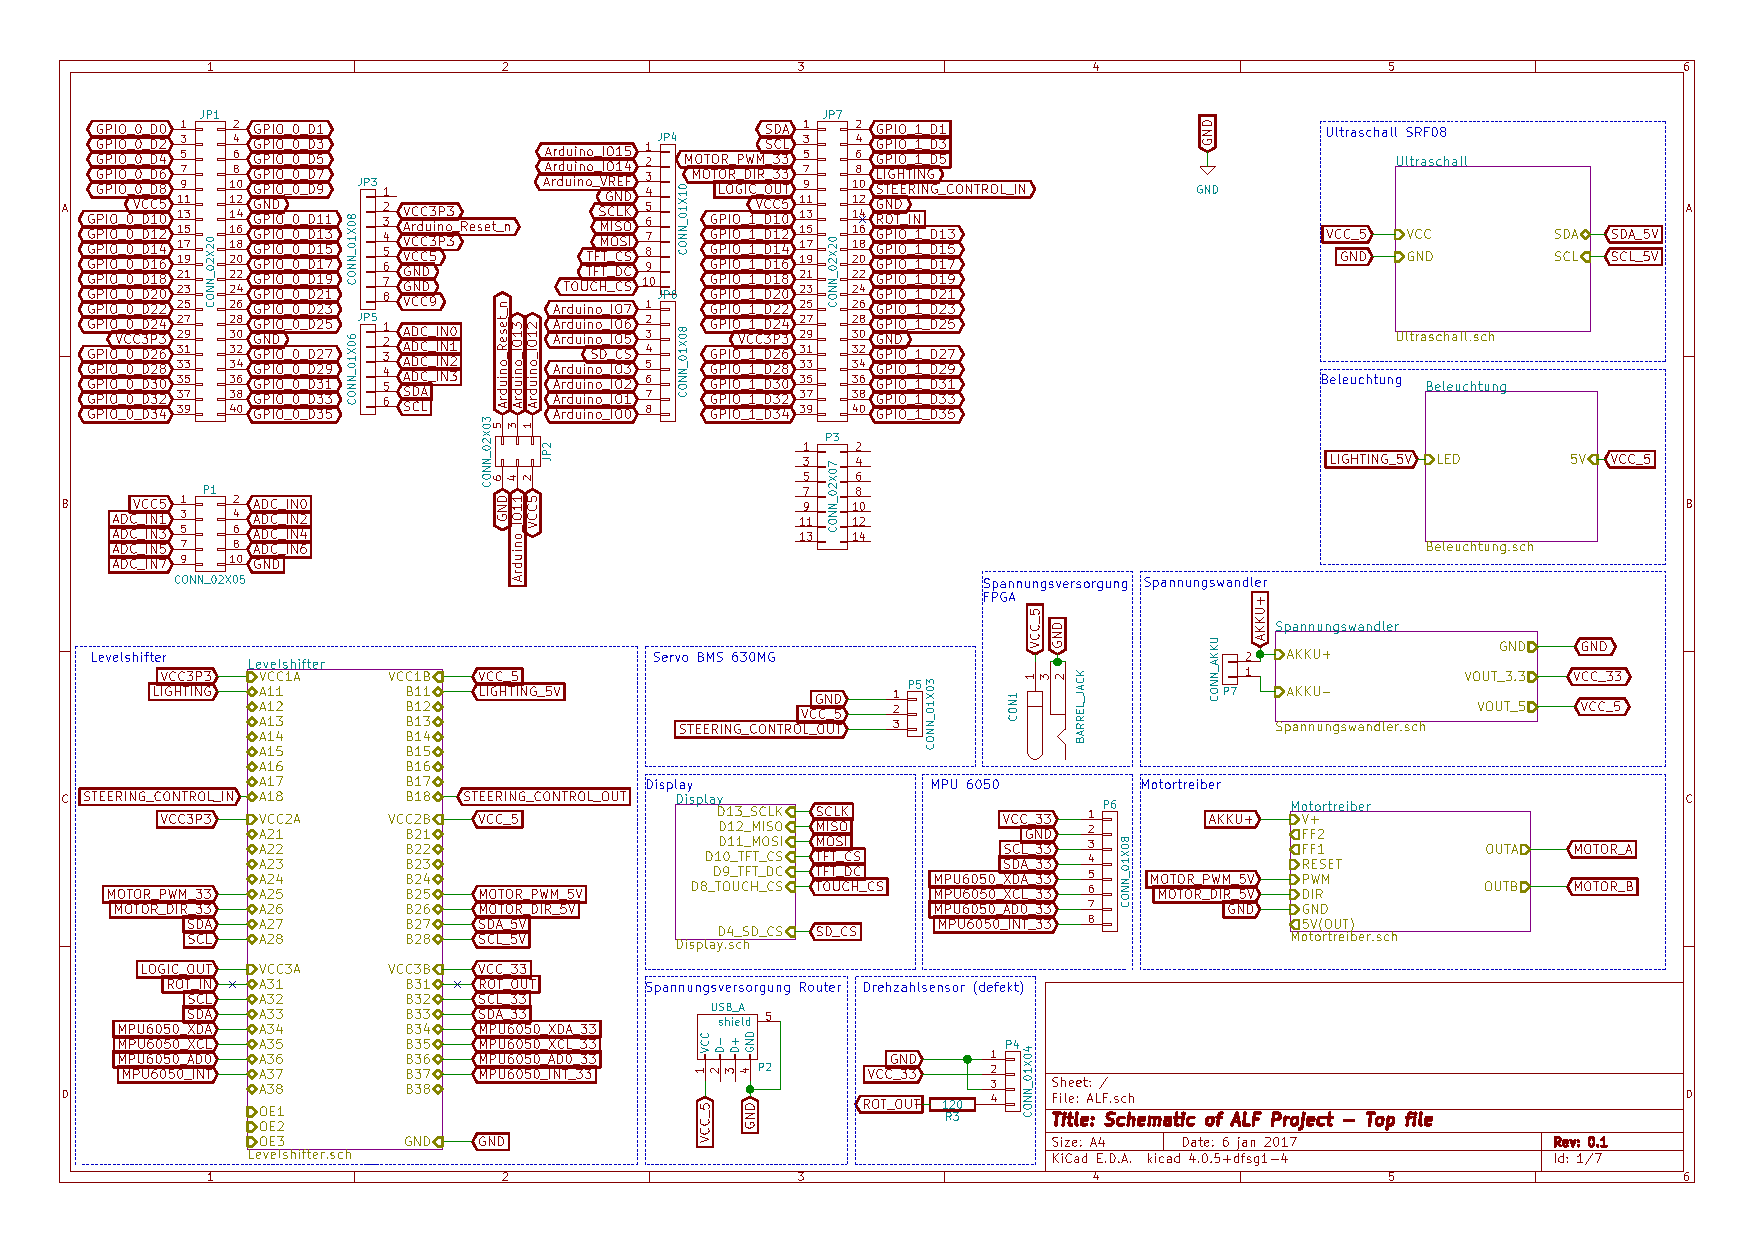
\includegraphics[angle=90, height=\textheight]{Abb/Garfield_Circuit.pdf}
	\caption{Schaltplan mit FPGA und verwendeter Peripherie}
	\label{Garfield_Circuit}
\end{figure}
Abbildung \ref{Garfield_Circuit} zeigt den erstellten Schaltplan des HSP. Dieser soll nachfolgend kurz beschrieben werden.\\
Alle ein- und ausgeheneden Signale mit Ausnahme der SPI Pins zur Ansteuerung des Displays (vgl. Abb. \ref{Garfield_Circuit} JP4) werden über Levelshifter geführt. Dies ermöglicht es zum einen alle Signale an die jeweils notwendigen Pegel anzupassen und zum anderen den maximalen vom FPGA bereitgestellten Strom nicht zu überschreiten. Dadurch ergeben sich die zwei Logikpegel 3,3V und 5V im System. Über den IIC Port werden alle Ultraschallsensoren und die MPU6050 angesprochen. Es wurden die internen pull-up Widerstände des IIC Ports aktiviert um dessen Funktionsfähigkeit sicherzustellen. Über den PWM Generator wird die Lenkung und der Motortreiber für die Geradeausfahrt angesteuert. Zur Ansteuerung der Beleuchtung und dem Setzen der Richtung des Motors werden einfache GPIO Pins benutzt. Der Schaltplan enthält zudem die Ansteuerung des Rotary Encoders zum Messen der Drehzahl des Motors. Da dieser jedoch unerwarteterweise nicht funktionsfähig war, sind die betrefenden Stellen im Schaltplan entsprechend gekennzeichnet.
\section{\ac{FPGA} Design}
Die Beschreibung des \ac{FPGA} wird, soweit möglich, mit dem Systemintegrationstool QSYS, das Teil der Quartus Toolchain ist, durchgeführt. Das Mapping zwischen QSYS-System und Pins wird klassisch in VHDL beschrieben. Das Top-Level-File des Systems ist \\ \texttt{FPGA\_Design/Garfield\_Design/Garfield.vhdl}. Dort wird das von QSYS erzeugt System und einige kleine \ac{IP}-Cores zusammengeführt und auf definierte Aus-/Eingänge geführt. Diese Ein-/Ausgänge werden dann über den \textit{Pin-Planner} auf die physikalischen Pins geführt.\\
Im Projektverzeichnis befinden sich alle Dateien, die für den \ac{FPGA} Teil relevant sind, unter \texttt{FPGA\_Design}. Die Struktur ab diesem Ordner ist wie folgt aufgebaut:
\begin{itemize}
	\item \texttt{Datasheets} - Einie Datenblätter und Application Notes zu dem \ac{FPGA} Teilprojekt
	\item \texttt{Garfield\_Design} - In diesem Ordner befinden sich die Quartus Projektdateien, Konfigurationsdateien und das QSYS Projekt.
	\item \texttt{ip\_extern} - Eine Sammlung von externen \ac{IP}-Cores, die im Projekt verwendet wurden. Es befinden sich dort nur die \ac{IP}-Cores, die nicht von Altera stammen oder nicht direkt in QSYS verfügbar sind.
	\item \texttt{ip\_intern} - Alle \ac{IP}-Cores, die für dieses Projekt entwickelt wurden.
	\item \texttt{output\_files} - In jedem Unterordner innerhalb dieses Ordners befinden sich \ac{FPGA} Images und die entsprechenden Konfigurationsdateien um ein Softwareprojekt dafür zu bauen.
\end{itemize}

Im folgenden werden die alle Systemkomponenten, die für das \Projectname-Projekt erzeugt wurden, beschrieben.

\section{\ac{IP}-Cores}
\label{IP-Cores}

\begin{figure}
	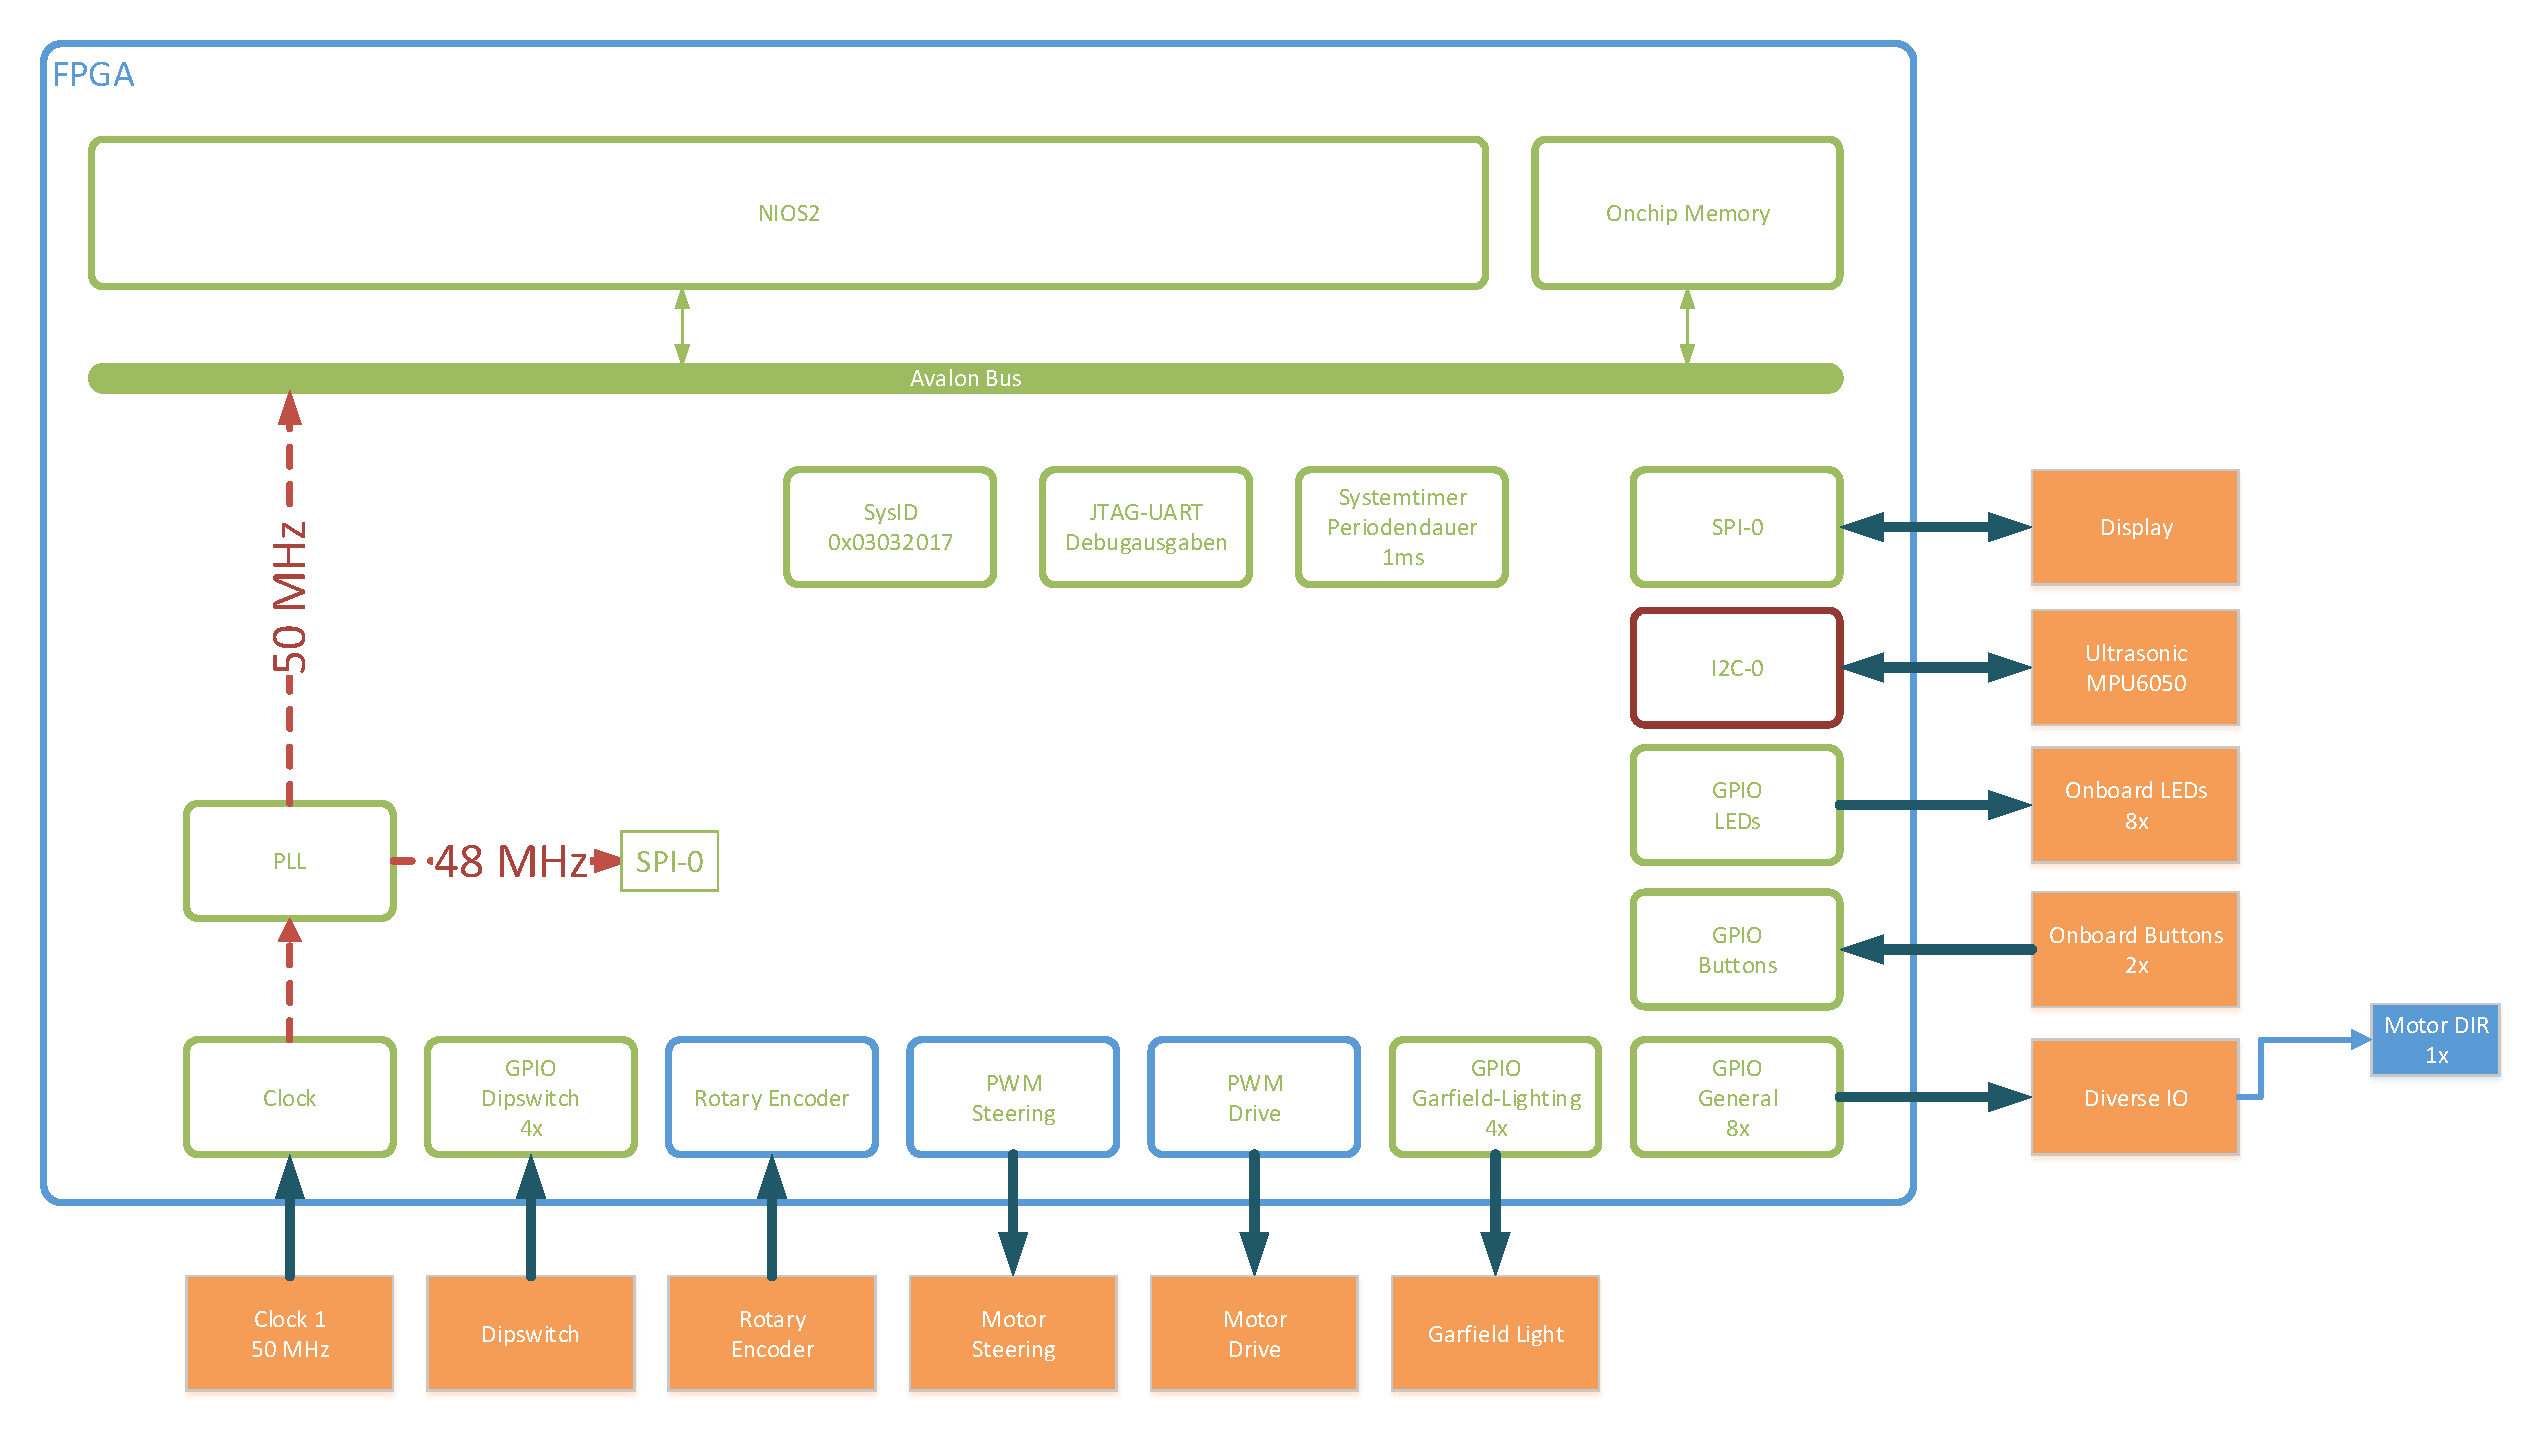
\includegraphics[angle=90, height=0.9\textheight]{Abb/Garfield_FPGA_Design_only_FPGA.pdf}
	\caption{Übersicht der (meisten) eingesetzten \ac{IP}-Cores. Die Abbildung verzichtet auf die Darstellung der Teile, die für die Kommunikation mit dem \ac{HPS} zuständig sind. Blau umrandet sind Cores, die im Rahmen des Projekts selbst progammiert wurden, grün diejenigen, die Teil der Altera Toolchain sind und rot externe IP-Cores von opencores.org}
	\label{FPGA_IP_FPGA_only}
\end{figure}

Abbildung \ref{FPGA_IP_FPGA_only} zeigt eine Übersicht der eingesetzten \ac{IP}-Cores und deren Verbindung zur Außenwelt. Ausgenommen sind die \ac{IP}-Cores, die für die Kommunikation mit dem \ac{HPS} benötigt werden. Die nachfolgende Tabelle beschreibt die Funktion der einzelnen IP-Cores im Detail und Besonderheiten dazu.

\begin{longtable}[ht]{|p{0.1\textwidth} | p{0.9\textwidth} |}
	\hline
	\textbf{Name} & \textbf{Beschreibung}\\
	\hline
	SPI-0 & Stellt einen SPI-Datenbus mit 24MHz Clock-Frequenz zur Verfügung. Es werden insgesamt 3 Chipselect Signale zur Verfügung gestellt, wobei aktuell nur eines für das Display benutzt wird. In der aktuellen Ausbaustufe wird nur das Display auf dem Arduino-Header auf dem FPGA angesteuert.\\ \hline
	I2C-0 & Stellt einen I2C Datenbus zur Verfügung. Der \ac{IP}-Core stammt von \href{opencores.org}{opencores.org} und wurde manuell integriert. Er stellt u.a. eine eine in Software änderbare Clock-Frequenz zur Verfügung und bindet die Ultraschallsensoren und die MPU-6050 an das System an.\\ \hline
	GPIO-X & Die verschiedenen GPIO Cores dienen dazu einfache Peripherie anzubinden. Dazu gehören die LEDs, die Dip-Switches, die Buttons und generische IOs, die im Projekt benötigt werden um z.B. die Drehrichtung des Motors einzustellen. \\ \hline
	PWM X & Die beiden PWM \ac{IP}-Cores erzeugen Signale zur Geschwindigkeitssteuerung und für den Lenkmotor. \\ \hline
	Rotary-Encoder & Der Rotary Encoder zählt die steigenden Flanken der NAME. Durch Abfragen des Ergebnisregisters in regelmäßigen festen Zeitinervallen kann die aktuelle Geschwindigkeit, die an den Rädern anliegt, gemessen werden. Leider funktioniert der NAME aktuell nicht mehr. Um das Signal zu nutzen müsste man die Hardware neu aufbauen bzw. ersetzen.\\ \hline
	Clock \& \ac{PLL} & Die externe Referenzclock taktet mit 50 MHz. Dieses Signal wird über eine \ac{PLL} allen beteiligten IP-Cores bereitgestellt. Auch die \ac{FPGA}-\ac{HPS} Bridges werden mit dem 50MHz Signal gespeist. Einzige Ausnahme bildet der SPI-0 Core. Um eine Frequenz von 24MHz zu erreichen (die maximale Frequenz mit der das Display angesprochen werden darf) wird ein vielfaches dieser Frequenz benötigt. Das nächsthöhere verfügbare vielfache der 24MHz sind 48MHz. Die selbst geschriebenen \ac{IP}-Cores sind von der Frequenz der \ac{PLL} abhängig. Erhöht man die Frequenz der \ac{PLL} auf z.B. 100MHz um mehr Laufzeit für einzelne Funktionen zur Verfügung zu haben, muss man die Frequenz in den \ac{IP}-Cores manuell anpassen! \\ \hline
	SysID & Mit der System ID (in Kombination mit einem Zeitstempel) kann man das Hardware Design eindeutig identifizieren. Dies ist hilfreich wenn mehrere Hardware- und Softwareversionen existieren, die parallel entwickelt werden. Um Zugriffsfehler auf Register oder ähnliches zu vermeiden, kann die Software die System-ID nutzen um Funktionen ab- bzw. zuzuschalten. \\ \hline
	JTAG-UART & Mit Hilfe dieses Cores kann man printf ähnliche Ausgaben für Debug-Ausgaben an einen angesteckten PC schicken. \\ \hline
	Systemtimer & Der Systemtimer ist ein kontinuierlich laufender Timer, der sich alle 1ms automatisch erhöht. Außerdem erzeugt er ein Interrupt, das FreeRTOS zur internen Zeitbestimmung nutzt. \\ \hline
	NIOS2 & Hierbei handelt es sich um eine Softcore-CPU. Diese wird von Altera zur Verfügung gestellt (inkl. Toolchain) und kann unbegrenzt benutzt werden (mit entsprechender Lizenz). Es handelt sich um eine 32-bit \ac{RISC} Architektur die durchaus eine weite Verbreitung im industriellen Umfeld genießt. Weiter Informationen dazu findet man unter \href{https://www.altera.com/products/processors/overview.html}{https://www.altera.com/products/processors/overview.html} \\ \hline
	Onchip Memory & Ein einfacher \ac{IP}-Core, der Speicherbausteine auf dem \ac{FPGA} nutzt um RAM(hier genutzt) oder ROM (nicht genutzt) zu erzeugen. Dieser Speicher kann dann von einem Prozessor (hier der NIOS2) als Instruktions- und Datenspeicher genutzt werden. In der aktuellen Ausbaustufe ist die Speichergröße mit 128kB angegeben. \\ \hline
\end{longtable}
\todo{NAME}

\begin{figure}
	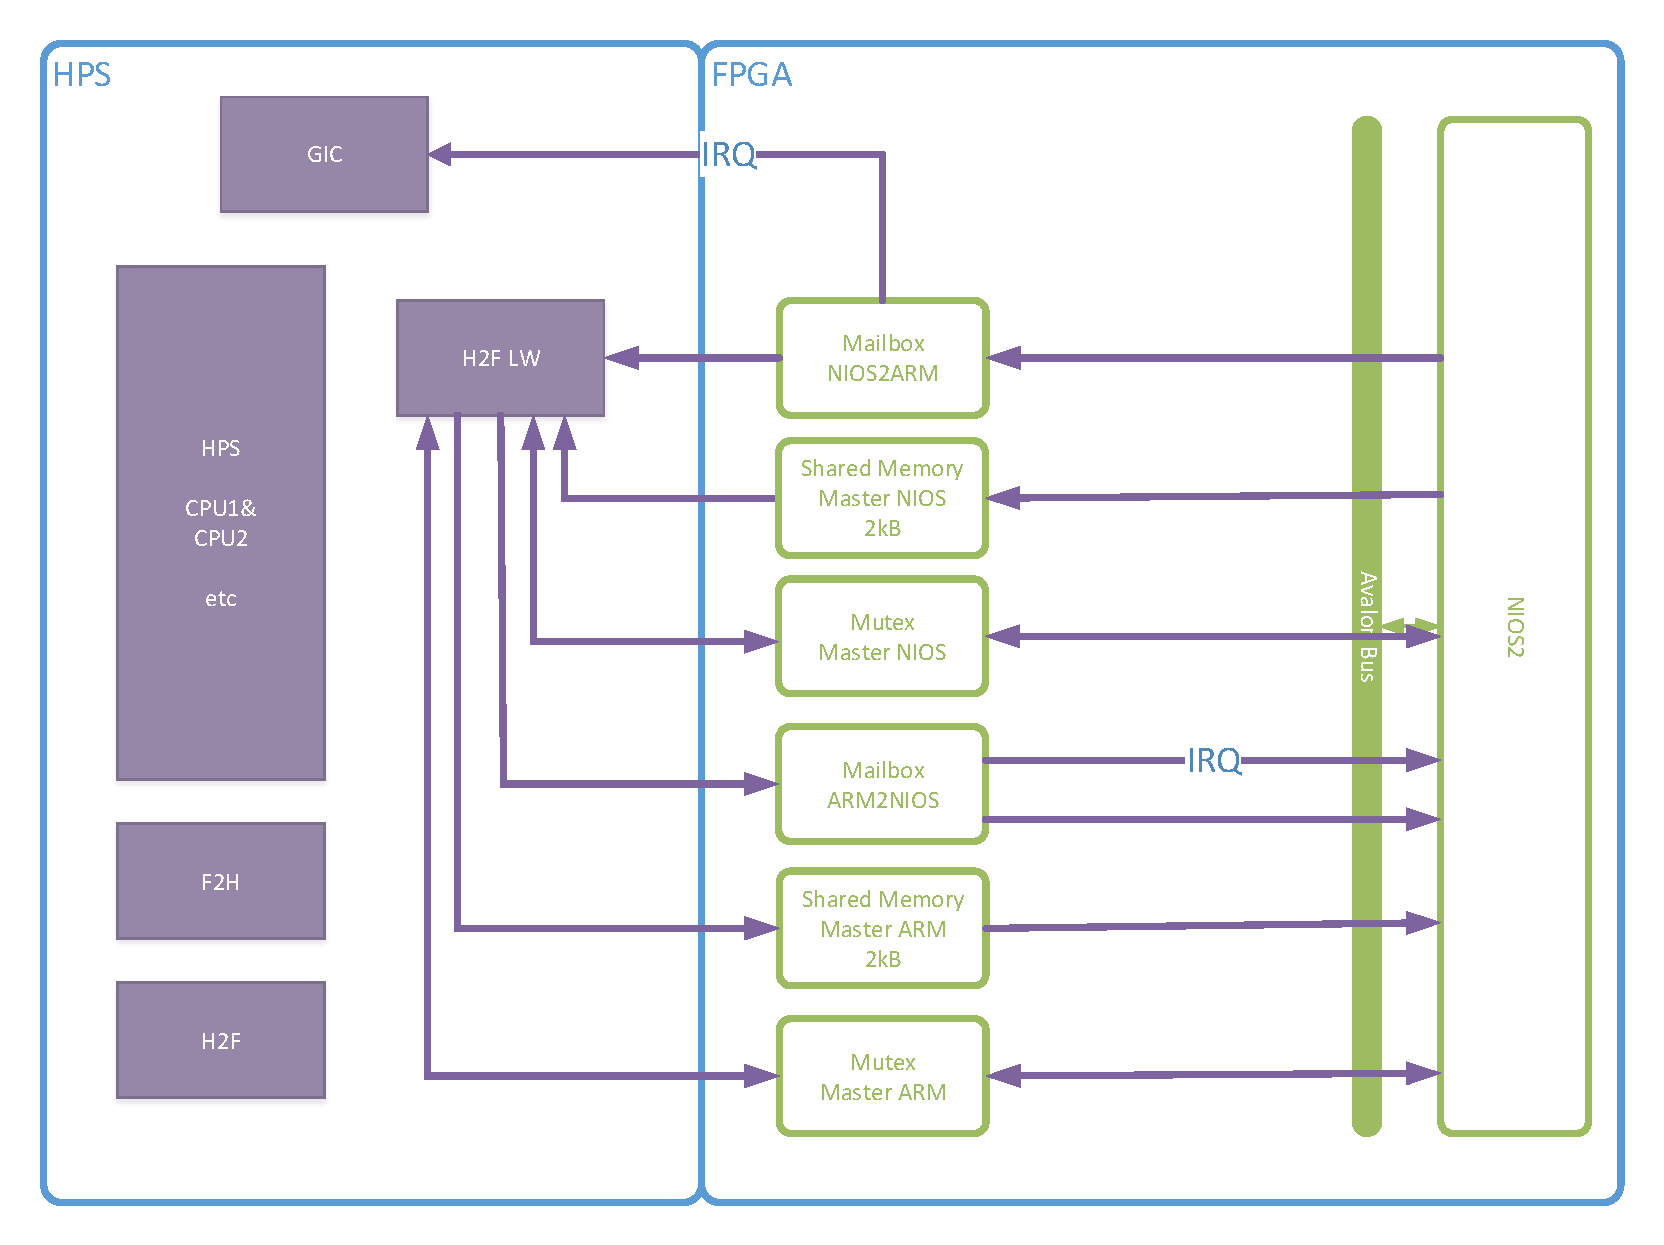
\includegraphics[angle=0, width=\textwidth]{Abb/Garfield_FPGA_Design_comm.pdf}
	\caption{\ac{IP}-Cores und deren Kontrollfluss, die an der Kommunikation zwischen NIOS2 und \ac{HPS} beteiligt sind.}
	\label{FPGA_IP_FPGA_comm}
\end{figure}

Abbildung \ref{FPGA_IP_FPGA_comm} zeigt die \ac{IP}-Cores, die für die Kommunikation zwischen \ac{FPGA} und \ac{HPS} benötigt/eingesetzt werden. Auf der linken Seite der Abbildung ist das \ac{HPS} System illustriert. Auf dieser Seite sind im wesentlichen drei Hardwareeinheiten an der Kommunikation beteiligt:
\begin{itemize}
	\item GIC - Der ARM \textit{General Interrupt Controller} : Dieser Controller ist ein sehr mächtiger Interrupt Controller, der u.a. die Interruptverarbeitung an die einzelnen CPUs verteilt. Insgesamt stehen 64 Interrupts zur Verfügung, die aus dem \ac{FPGA} heraus ausgelöst werden können. Auf dem eingesetzten Cyclone V beginnen diese mit der Interrupt ID 72 vom GIC. Genauere Informationen zum GIC kann man entweder auf der Homepage von ARM oder \cite{Using_GIC} erhalten.
	\item H2F LW - Die \ac{HPS}2\ac{FPGA} Leightweight Bridge : Dies ist eine der drei Bridges, mit denen zwischen \ac{FPGA} und \ac{HPS} kommuniziert werden kann. Dies ist keine High-Performance Bridge, es ist aber keine großen Änderungen notwendig, das System auf eine der anderen Bridges umzubauen. Diese Bridge \textbf{muss} aktiviert werden, bevor über sie kommuniziert werden kann. Ist die Bridge nicht aktiviert, treten \textit{Segmentation Faults} auf (kein gültiger Speicherbereich). Im Prinzip befindet sich \textquotedblleft hinter\textquotedblright der Bridge ein Speicherbereich, der durchgehend addressiert werden kann um direkt in Register zu schreiben. Auch lesende Zugriffe daraus können erfolgen \cite{FPGA_Workshop}.
	\item CPUs - Die ARM A9 Applikationsprozessoren dienen zur Verarbeitung der Interrupts bzw. zum triggern der einzelnen IP-Cores.
\end{itemize}

Es folgt eine Beschreibung der \ac{IP}-Cores, die für die Kommunikation gebraucht werden. Da die Kommunikationseinheiten in beide Richtungen analog aufgebaut sind, beschränkt sich die Beschreibung auf einen Richtung:
\begin{itemize}
	\item Mailbox X2Y : Die Mailbox ist ein einfacher IP-Core der Nachrichten von einem Buspartner (X, z.B. NIOS2) einem anderen Buspartner (Y, z.B. ARM) zur Verfügung stellt. Es gibt also einen Transmitter und einen Receiver. Beide sind über eigene Interfaces (und damit über ihren eigenen Addressbereich) an die Mailbox angeschlossen. Die Nachrichtenübermittlung erfolgt mit Hilfe von zwei Registern:
	\begin{itemize}
		\item Command Register - Dieses Register kann vom Empfänger nur gelesen werden. Es dient dazu, ein Kommando oder Nachricht an den Empfänger zu senden. Ein schreibender Zugriff auf dieses Register vom Sender löst das zugehörige Interrupt aus, dass vom Empfänger verarbeitet werden muss.
		\item Pointer Register - In diesem Register wird die Addresse, in der die eigentliche Nachricht im Speicher steht, übertragen. Sollen nur ganz kleine Nachrichten (4 oder 8 Bytes) übertragen werden, kann man das Pointer und Command Register dazu benutzen, die Nachricht zu übertragen. In diesem Projekt wird aber die eigentliche Nachricht im Shared Memory übertragen, in der Mailbox nur die Addresse im Shared Memory und ein Kommando im Command Register
	\end{itemize}
	Eine detailierte Beschreibung des Cores findet sich unter \cite[470ff]{embedded_guide}
	\item Shared Memory Master X - Dieser Speicher, der wie der Arbeitsspeicher des NIOS2 direkt im \ac{FPGA} synthetisiert wird, dient der Nachrichtenübermittlung. Dort werden die Nutzdaten einer Nachricht von X reingeschrieben und können zu einem späteren Zeitpunkt vom Empfänger Y ausgelesen werden. Es wurde sich bewusst dazu entschieden zwei Shared Memory zu benutzen um eine jegliche Kollision zu vermeiden bzw. zu vereinfachen. Die Größe beider Speicherbereiche beträgt jeweils 2kB. Dies reicht für die aktuellen Nachrichten leicht aus. Zu einem späteren Zeitpunkt können die Bereiche auch noch vergrößert werden, sollte der Speicher nicht groß genug sein Nachrichten zu übertragen.
	\item Mutex Master X - Dies ist ein spezieller \ac{IP}-Core, der auch als Teil des Altera \ac{IP}-Core Katalogs zur Verfügung stellt. Dieser hat nur ein Register, das hier betrachtet werden soll und erlaubt einen atomaren Mutex Zugriff auf geteilte Resourcen. Die geteilte Resource, die über diesen Mutex gesperrt wird ist der zugehöriger Shared-Memory. Die Referenz für diesen Core ist ebenfalls \cite[319ff]{embedded_guide}. Das Register besteht aus zwei Teilen: die oberen 16 Bit werden als Speicherplatz für die CPU-ID (der NIOS2 hat die ID 0x03, der ARM immer 0x01) benutzt. In die unteren 16 Bit kann ein beliebiger Wert gespeichert werden. Ein lesender Zugriff auf den Mutex ist immer möglich. Ein schreibender Zugrif ist nur möglich wenn
	\begin{itemize}
		\item Die CPU-ID mit der CPU-ID übereinstimmt, dessen Wert man in das Register schreiben will.
		\item (oder) Der Wert (untere 16-Bit) Null ist.
	\end{itemize}
	Man kann also nur schreibend auf den Mutex zugreifen, wenn einem der Mutex bereits gehört oder der Mutex frei (=0) ist. Nach einem schreibenden Zugriff muss der Registerwert mit dem Wert der geschrieben wurde verglichen werden. Stimmen beide Werte überein, hat der Schreiber den Mutex gelockt, andernfalls ist der atomare Lock fehlgeschlagen.
\end{itemize}

\section{Address-Map}

\begin{figure}
	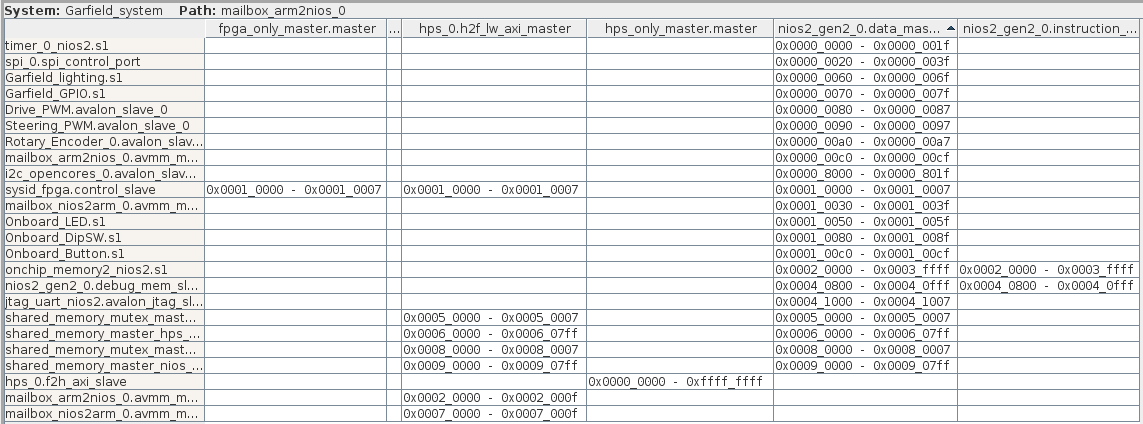
\includegraphics[width=\textwidth]{Abb/Address_Map.png}
	\caption{Übersicht über die Addressen und Addressbereiche im System}
	\label{FPGA:AddrMap}
\end{figure}

Abbildung \ref{FPGA:AddrMap} zeigt die Addressen die im System benutzt werden und den zugehörigen Addressbereich der verfügbar ist. Diese Addressmap ist auch im QSYS-Projekt des Projektes verfügbar.

\section{Eigenentwickelte \ac{IP}-Cores}

\subsection{Der PWM-Generator} generiert ein PWM Signal auf die Ausgabeleitung. Der Registerzugriff ist in Tabelle \ref{hw:pwm} dargestellt

\begin{table}
\begin{longtable}[]{@{}c|l|c|c|l@{}}
	\textbf{Bit} & \textbf{Name} & \textbf{Access} & \textbf{Reset Value} &
	\textbf{Description}\tabularnewline

	\endhead
	\texttt{7\ ...\ 0} & control & RW & 0 & sets the dutycylce of the PWM
	signal generator\tabularnewline
	\texttt{31\ ...\ 7} & - & R & 0 & not used\tabularnewline

\end{longtable}
\caption{Registermap des PWM Cores}
\label{hw:pwm}
\end{table}

\subsection{Der Rotary Encoder} \ac{IP}-Core kann steigende Flanken von einer externen Flanke zählen, hat ein auslesbares Ergebnisregister (siehe \ref{hw:rotary:result})und ein Controlregister (siehe \ref{hw:rotary:control}).

\begin{table}
\begin{longtable}[]{@{}clccl@{}}
	\begin{minipage}[b]{0.13\columnwidth}\centering\strut
		\textbf{Bit}\strut
		\end{minipage} & \begin{minipage}[b]{0.08\columnwidth}\raggedright\strut
		\textbf{Name}\strut
		\end{minipage} & \begin{minipage}[b]{0.12\columnwidth}\centering\strut
		\textbf{Access}\strut
		\end{minipage} & \begin{minipage}[b]{0.17\columnwidth}\centering\strut
		\textbf{Reset Value}\strut
		\end{minipage} & \begin{minipage}[b]{0.15\columnwidth}\raggedright\strut
		\textbf{Description}\strut
		\end{minipage}\tabularnewline
		\endhead
		\begin{minipage}[t]{0.13\columnwidth}\centering\strut
			\texttt{0}\strut
			\end{minipage} & \begin{minipage}[t]{0.08\columnwidth}\raggedright\strut
			enable\strut
			\end{minipage} & \begin{minipage}[t]{0.12\columnwidth}\centering\strut
			RW\strut
			\end{minipage} & \begin{minipage}[t]{0.17\columnwidth}\centering\strut
			0\strut
			\end{minipage} & \begin{minipage}[t]{0.15\columnwidth}\raggedright\strut
			Enable bit for the core\strut
			\end{minipage}\tabularnewline
			\begin{minipage}[t]{0.13\columnwidth}\centering\strut
				\texttt{1}\strut
				\end{minipage} & \begin{minipage}[t]{0.08\columnwidth}\raggedright\strut
				clear\strut
				\end{minipage} & \begin{minipage}[t]{0.12\columnwidth}\centering\strut
				W\strut
				\end{minipage} & \begin{minipage}[t]{0.17\columnwidth}\centering\strut
				0\strut
				\end{minipage} & \begin{minipage}[t]{0.15\columnwidth}\raggedright\strut
				Clear bit. clears the result register and set it to 0; Must not be
				manually set to 0 after clearing. With the next rising edge of the clock
				it goes down on itself.\strut
				\end{minipage}\tabularnewline
				\begin{minipage}[t]{0.13\columnwidth}\centering\strut
					\texttt{2}\strut
					\end{minipage} & \begin{minipage}[t]{0.08\columnwidth}\raggedright\strut
					reset\strut
					\end{minipage} & \begin{minipage}[t]{0.12\columnwidth}\centering\strut
					W\strut
					\end{minipage} & \begin{minipage}[t]{0.17\columnwidth}\centering\strut
					0\strut
					\end{minipage} & \begin{minipage}[t]{0.15\columnwidth}\raggedright\strut
					Resets the whole core and set all values to default. At a read
					operation, it is always 0\strut
					\end{minipage}\tabularnewline
					\begin{minipage}[t]{0.13\columnwidth}\centering\strut
						\texttt{15\ ...\ 3}\strut
						\end{minipage} & \begin{minipage}[t]{0.08\columnwidth}\raggedright\strut
						not accessable\strut
						\end{minipage} & \begin{minipage}[t]{0.12\columnwidth}\centering\strut
						-\strut
						\end{minipage} & \begin{minipage}[t]{0.17\columnwidth}\centering\strut
						0\strut
						\end{minipage} & \begin{minipage}[t]{0.15\columnwidth}\raggedright\strut
						-\strut
						\end{minipage}\tabularnewline
						\begin{minipage}[t]{0.13\columnwidth}\centering\strut
							\texttt{16}\strut
							\end{minipage} & \begin{minipage}[t]{0.08\columnwidth}\raggedright\strut
							error\strut
							\end{minipage} & \begin{minipage}[t]{0.12\columnwidth}\centering\strut
							R\strut
							\end{minipage} & \begin{minipage}[t]{0.17\columnwidth}\centering\strut
							0\strut
							\end{minipage} & \begin{minipage}[t]{0.15\columnwidth}\raggedright\strut
							Indicates an error within the counting process. You should reset the
							core!\strut
							\end{minipage}\tabularnewline
							\begin{minipage}[t]{0.13\columnwidth}\centering\strut
								\texttt{31\ ...\ 17}\strut
								\end{minipage} & \begin{minipage}[t]{0.08\columnwidth}\raggedright\strut
								not accessable\strut
								\end{minipage} & \begin{minipage}[t]{0.12\columnwidth}\centering\strut
								-\strut
								\end{minipage} & \begin{minipage}[t]{0.17\columnwidth}\centering\strut
								0\strut
								\end{minipage} & \begin{minipage}[t]{0.15\columnwidth}\raggedright\strut
								-\strut
								\end{minipage}\tabularnewline

\end{longtable}
\caption{Registermap des Controlregisters des Rotary Encoder}
\label{hw:rotary:control}
\end{table}

\begin{table}
	\begin{longtable}[]{@{}clccl@{}}
		\textbf{Bit} & \textbf{Name} & \textbf{Access} & \textbf{Reset Value} &
		\textbf{Description}\tabularnewline
		\endhead
		\texttt{31\ ...\ 0} & result & R & 0 & Result of the counting
		process\tabularnewline
	\end{longtable}
	\caption{Registermap des Ergebnisregisters des Rotary Encoder}
	\label{hw:rotary:result}
\end{table}

\chapter{Software}
Die Software unterteilt sich insgesamt in 3 Teile.
\begin{itemize}
 \item Headquarter (HQ): Linux System das mit dem Fahrzeug über WLAN kommuniziert
 \item ARM: Linux ARM System, dass die Netzwerkaufgaben, sprich Kommunikation, mit dem HQ übernimmt
 \item NIOS: VHDL Core, der sonstige Periphere anspricht auf dem ein Echtzeitbestriebsystem (FreeRTOS) läuft. Die Software hiervon setzt sich zusammen aus /Software/common/ARM\_NIOS\_HQ/, /Software/common/ARM\_NIOS und Software/Software\_NIOS2/*.
\end{itemize}

\section{HQ}
Nachfolgend wird die Umsetzung der Headquarter-Software \glqq Garfield Control\grqq{} beschrieben. Diese ermöglicht sowohl die Steuerung des Fahrzeuges, als auch die Visualisierung der vom Fahrzeug bzw. den angebrachten Sensoren erfassten Daten.

\subsubsection{Funktionalitäten}

Zur Herstellung der Verbindung zum Comm Gateway lassen sich die verwendete IP-Adresse und der Port im Einstellungsdialog festlegen. Auch die Verbindung zu einem Playstation 3 Controller lässt sich dort definieren. Durch Verlassen des Einstellungsdialoges mit dem OK-Button werden alle Einstellungen gespeichert und anschließend versucht eine Verbindung zum Controller herzustellen. Hat dies nicht geklappt, wird eine entsprechende Nachricht in der Statusleiste angezeigt. Durch Aktivieren der Debugausgaben lässt sich außerdem die Funktionalität der Steuerung mithilfe des Controllers testen. Im Anschluss lässt sich die Socketverbindung zum Comm Gateway durch Klicken des Connect-Buttons starten.

Ist eine Verbindung zum Comm Gateway hergestellt, lässt sich das Fahrzeug steuern und alle empfangenen Daten visualisieren. Dies wird nachfolgend kurz erläutert.

\paragraph{Die Steuerung} des Fahrzeuges ist am komfortablesten durch Benutzung des laboreignen Playstation 3 Controller möglich. Zudem lässt es sich durch Benutzung der Tastatur oder der direkten Bedienung der GUI Elemente mit der Maus bedienen. Dabei sind folgende Befehle möglich:

\begin{itemize}
	\item Die Geschwindigkeit in Fahrtrichtung (vorwärts oder rückwärts) lässt sich am Controller durch Betätigung von R2 (vorwärts) oder L2 (rückwärts) setzen. Dabei werden die vom Controller übermittelten Geschwindigkeitswerte in einen Wertebereich von 0 - 255 übersetzt und anschließend zusammen mit der Richtungsangabe übertragen. Durch Drücken der Taste W (vorwärts) oder S (rückwärts) auf der Tastatur oder einen Klick auf den entsprechenden Button der Anwendung lässt sich die maximale Geschwindigkeit ebenfalls setzen.
	
	\item Die Lenkung des Fahrzeuges lässt sich durch Bedienung des linken Sticks auf dem Controller steuern. Dabei werden Werte zwischen -90° und 90° versendet. Durch Verwendung der Tasten D oder A oder Klicken auf den entsprechenden Button lässt sich außerdem der maximale Lenkeinschlag setzen.
	
	\item Die am Fahrzeug angebrachte Beleuchtung lässt sich durch Betätigung des Triangle-Buttons, Klicken auf L oder einen Klick auf die entsprechende Checkbox in der Anwendung aktivieren oder deaktivieren.
	
\end{itemize}

\paragraph{Die Visualisierung} der vom Fahrzeug übertragenen Daten umfasst neben der durch den rotary encoder gemessenen Geschwindigkeit, alle Daten der MPU6050, wie die Temperatur sowie Beschleunigung und Neigung des Fahrzeuges an allen 3 Achsen. Diese empfangenen Werte werden in der Applikation entsprechend dargestellt. Bis auf die Beschleunigung, welche durch einen sich der jeweiligen Achse anpassenden Punkt in einem Koordinatensystem dargestellt wird, werden alle Werte in Textausgabefeldern angezeigt.

\subsubsection{Umsetzung}
Die Anwendung Garfield Control wurde mithilfe von Qt für Linux entwickelt. Alle für die Socketverbindung gemeinsam genutzten Funktionen sind unter \texttt{Software/common/ARM\_HQ} bzw. \texttt{Software/common/ARM\_NIOS\_HQ} abgelegt. Die eigenständigen Softwarebestandteile sind unter \texttt{Software/Software\_HQ/Garfield\_Control} vorhanden. Zur einfachen Benutzung der Anwendung wurden alle notwendigen Bibliotheken und Plugins mithilfe von \href{https://github.com/probonopd/linuxdeployqt}{linuxdeployqt} zusammengefügt und als zip-Datei im Repository abgelegt. Somit lässt sich Garfield Control auch ohne eine Installation von Qt Paketen benutzen.\\
Die Verbindung zu einem Playstation 3 Controller wurde mithilfe einer API, welcher der Device Name übergeben wird, umgesetzt (\href{https://github.com/drewnoakes/joystick}{Github Repository}). Ist ein Controller mit der Anwendung verbunden, so wird dieser alle 20ms nach aufgetretenden Events abgefragt.\\
Ebenfalls alle 20ms wird die Aktualisierung der Visualisierung der Beschleunigungswerte durchgeführt. Diese zyklischen Aufgaben werden unter zuhilfename von QTimern gestartet. Dazu lässt sich der Ablauf der Timer mit dem Aufruf der entsprechenden Methode verknüpfen.\\
Wurde eine Socketverbindung mit dem Comm Gateway hergestellt, so werden zwei seperate Threads gestartet, welche alle 20ms versuchen Informationsdaten zu empfangen, bzw. Steuerungsbefehle zu senden. Dazu wurden die gemeinsam verwendeten Klassen \texttt{Alf\_Drive\_Info} und \texttt{Alf\_Drive\_Command} benutzt, sodass sichergestellt ist, dass alle beteiligten Kommunikationspartner die gleiche Datenstruktur benutzen können.

\section{ARM}
\todo{Comm Gateway beschreiben}

\subsubsection{Mailbox Kommunikation ARM $\leftrightarrow$ NIOS2}
Die Kommunikation über die in das \ac{FPGA} programmierte Mailbox (siehe \ref{IP-Cores}) wird über eine abstrakte Klassenimplementierung in C++ dargestellt. \todo{Name, Pfad?}
Die Klasse stellt einige \textit{Write} und \textit{Read} Funktionen zur Verfügung, die mit verschiedenen Objekten umgehen können. Durch dieses Vorgehen ist sichergestellt, das der Aufrufer als Übergabeparameter nur bestimmte Objekte (die sauber definiert sind) übergegeben werden können, die auch verarbeitet werden können. Die Kommunikation erfolgt asynchron und ist intern gepuffert. Die Klasse dient als Abstraktionsschicht in beide Richtungen. Sowohl die Empfangsrichtung als auch die Senderichtung werden über die Klasse abgebildet, sodass der Aufrufer keinerlei interne Informationen über die Hardware und die Implementierung haben muss.
Nachfolgend werden die beiden wesentlichen Operationen (\textit{Write} und \textit{Read}) dargestellt und beschrieben.

\begin{figure}
	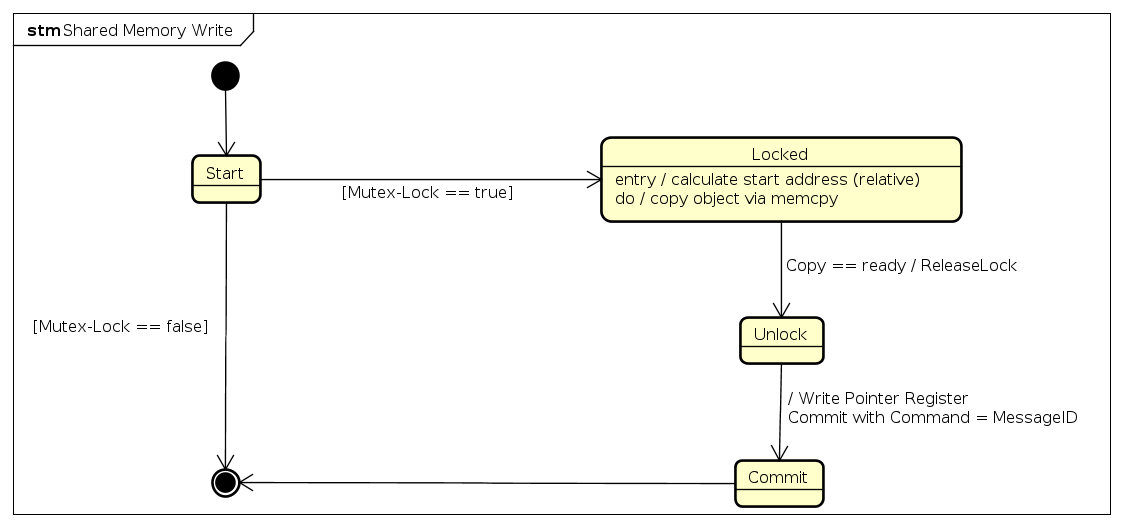
\includegraphics[width=\textwidth]{Abb/Shared_mem_Write.png}
	\caption{Schreibvorgang in den Shared Memory}
	\label{Software:Arm:SharedMemWrite}
\end{figure}

\paragraph{Write}
Der schreibende Zugriff auf den Shared Memory ist in Abbildung \ref{Software:Arm:SharedMemWrite} illustriert und hat einen einfachen Ablauf. Nachdem sich der Schreiber den Lock auf den Shared Memory über den Mutex Core geholt hat kann er Daten in diesen Bereich schreiben. Der Speicher wird dabei linear durchlaufen. Der Speicher wird dabei wie ein Ringspeicher behandelt. Ist am oberen Ende des Speichers nicht mehr genug Platz für die neue Nachricht wird wieder bei der relativen Addresse Null angefangen zu schreiben. Sind alle Daten in den Speicher geschrieben wird der Mutex wieder freigelassen. Im Speicher steht jetzt ein Abbild des Objekts, das übertragen werden soll. Es werden also nur Nutzdaten in den Speicher geschrieben. Anschließend wird die Startaddresse der Daten in das Pointer Register der Mailbox geschrieben. In das Command Register wird die eindeutige Nachrichten ID, die innerhalb des Garfield Projekts definiert ist, geschrieben. Dieser Schreibvorgang ist die letzte Instruktion zum Nachrichtenaustausch aus Sendersicht.

\paragraph{Read}
Der lesende Zugriff auf den Shared Memory ist komplizierter und unterteilt sich in zwei Abschnitte.\\

Der erste Teil der lesenden Kommunikation besteht aus dem \textbf{Interrupt}. Von dem Mailbox \ac{IP}-Core wird bei einem schreibenden Zugriff auf das Command Register automatisch ein Interrupt erzeugt. Innerhalb des \textit{ReadInterruptHandler} wird nicht der Shared Memory ausgelesen, sondern nur die Nachricht aus der Mailbox gespeichert. Die Klasse hält zusätzlich zu jedem Objekt, das verschickt bzw. empfangen werden soll einen kleinen Ringpuffer. Dieser dient dazu, die Addressen der Objekte im Shared Memory zu puffern. Tritt nun das Interrupt auf, wird zuerst das Pointer Register zwischengespeichert. Anschließend wird das Command Register, in dem der Nachrichtentyp übertragen wird, ausgelesen und anhand des Nachrichtentyps die Addresse des Pointer Registers in den passenden Puffer geschrieben. Dieses Vorgehen sorgt dafür, dass diese Funktion, die in einem Interrupthandler ausgeführt wird, sehr schnell wieder beendet ist.\\

Der zweite Teil besteht aus einem \textbf{Hintergrundtask} der zyklisch durchlaufen wird. Innerhalb dieses Task werden die Werte eines Objekts, die ausgelesen werden sollen, über eine \textit{Read} Funktion bei Bedarf überschrieben. Bei Bedarf deswegen, weil die Werte nur überschrieben werden, wenn aktuellere Werte im Shared Memory stehen. Sind aktuelle Werte verfügbar, ist der Klasseninterne Ringpuffer, der die Addressen für die Nutzdaten enthält, nicht leer. Es wird über die Addresse aus dem Shared Memory gelesen und anschließend diese Nachricht (also die Addresse) aus dem Ringpuffer entfernt.

\subsubsection{\ac{HPS} Startvorgang und Software}
Der folgende Abschnitt beschreibt die Bestandteile die für den Betrieb des ARM Dualcore notwendig sind und wie diese konfiguriert und kompiliert werden.\\

\begin{figure}
	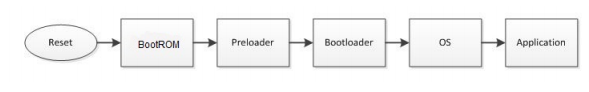
\includegraphics[width=\textwidth]{Abb/Booting.png}
	\caption{Typsicher Bootvorgang des ARM A9 Dualcore Prozessors \cite{arm_booting}}
	\label{Software:ArmBooting}
\end{figure}

Eine sehr gute und übersichtliche Beschreibung des Bootvorgangs der A9 Kerne ist in \cite{arm_booting} beschrieben. Der im \Projectname Projekt verwendeter Bootvorgang ist in Abbildung \ref{Software:ArmBooting} dargestellt. Die ersten beiden Schritte (BootRom, Preloader) sollen hier nicht weiter beschrieben werden da keine manuelle Anpassung daran notwendig ist. Als Referenz für den Buildvorgang des gesamten Systems diente \href{https://eewiki.net/display/linuxonarm/DE0-Nano-SoC+Kit}{https://eewiki.net/display/linuxonarm/DE0-Nano-SoC+Kit}. Eine komplette Kopie des Tutorials befindet sich auch im Projektverzeichnis unter \todo{Pfad}. Wenn Änderungen an der im Tutorial beschriebenden Vorgehensweise notwendig sind werden diese erwähnt.

\paragraph{Als Bootloader} kommt der beliebte U-Boot \footnote{\href{https://www.denx.de/wiki/U-Boot}{https://www.denx.de/wiki/U-Boot}} in einer leicht angepassten Variante zum Einsatz. Wie im Tutorial beschrieben werden einige Startvariablen(unter anderem das zu ladende Linux Device Tree Binary) hinzugefügt um von der SD Karte zu booten. U-Boot lädt nach dem Start dann automatisch zunächst den

\paragraph{Linux Device Tree} Der Linux Device Tree ist ein Bestandteil des Linux Kernels um eine Abstraktionsschicht zwischen Hardware (Pinouts, Speicher, Interrupts) und dem Linux Kernel zu schaffen. Durch Einsatz des Device Tree kann ein gleiches Kernel Binary auf verschiedenen Hardwareversionen und sogar komplett verschiedenen Boards benutzt werden. Der Device Tree ist eine textuelle Beschreibung der Hardware die kompiliert wird und dem Kernel beim Startvorgang übergeben wird. Ein Auszug aus einem solchen Device Tree zeigt der Code \ref{Software:DeviceTree}. Die Spezifikation des Device Trees kann man unter \href{http://www.devicetree.org/specifications/}{http://www.devicetree.org/specifications/} einsehen.

\begin{lstlisting}[caption={[Auszug aus socfpga.dtsi]Auszug aus socfpga.dtsi \cite[Version~4.7, \texttt{arch/arm/boot/dts/socfpga.dtsi}]{Linux_Kernel}}, label=Software:DeviceTree]
cpus {
	#address-cells = <1>;
	#size-cells = <0>;
	enable-method = "altr,socfpga-smp";
	
	cpu@0 {
		compatible = "arm,cortex-a9";
		device_type = "cpu";
		reg = <0>;
		next-level-cache = <&L2>;
	};
	cpu@1 {
		compatible = "arm,cortex-a9";
		device_type = "cpu";
		reg = <1>;
		next-level-cache = <&L2>;
	};
};
\end{lstlisting}

\begin{lstlisting}[caption={[Änderungen am Device Tree]Notwendige Änderungen am Device Tree}, label=Software:DevTreeGarfield]
&fpga_bridge0 {
	bridge-enable = <1>;
};

&fpga_bridge1 {
	bridge-enable = <1>;
};

&fpga_bridge2 {
	bridge-enable = <1>;
};

/* we are extending the soc device with a specific interrupt! */
/{
	soc {
		mbox_rx: mailbox@0x00070000 {
			compatible = "altr,mailbox-1.0";
			reg = <0x70000 0x8>;
			interrupt-parent = < &intc >;
			interrupts = <GIC_SPI 60 4>;
			#mbox-cells = <1>;
		};
	};

};

\end{lstlisting}
Die Änderungen, die für den Device Tree im \Projectname Projekt nötig sind, sind im Codeausschnitt \ref{Software:DevTreeGarfield} gezeigt. Es existiert außerdem eine patch-Datei, mit der der geänderte Device Tree direkt in die heruntergeladenen Kernelsourcen gepatcht und kompiliert werden kann. Die vorgenommen Änderungen ergeben sich wie folgt
\begin{itemize}
	\item fpga\_brigdes - Durch die hinzugefügten Einträge \texttt{fpga\_bridgeX} werden die verschieden verfügbaren (Achtung: Ist nur für Kernel Version 4.7 so gültig, ältere Kernel haben u.U. weniger verfügbare Bridges) Bridges beim Laden des Device Tree aktiviert.
	\item mbox\_rx - Mit diesem Eintrag wird das Interrupt, ausgelöst durch den Mailbox \ac{IP}-Core (siehe \ref{IP-Cores}) als verfügbare Hardwareeinheit dem Kernel bekanntgemacht. Interessante Attribute sind
	\begin{itemize}
		\item \texttt{@} - Die Zahl nach dem @ entspricht der Physikalischen Addresse der Mailbox. Da die Adresse im weiteren Verlauf nicht verwendet wird ist der exakte Wert nicht von Bedeutung.
		\item \texttt{compatible} - Mit diesem Attribut wird dem Interrupt ein Name gegeben. Wäre im Kernel ein generischer Hardwaretreiber für diese Mailbox vorhanden könnte dieser zur Verarbeitung genutzt werden. Wichtig für das Projekt ist der Name trotzdem, da damit das Zuordnen der Interrupt-Service-Routine zu dem Interrupt geschieht.
		\item \texttt{interrupt-parent} - Damit wird der Interrupt Controller (in unserem Fall der ARM GIC, der in einer inkludierten Beschreibungsdatei beschrieben wird) identfiziert, der das Interrupt aufnimmt und die weitere Abarbeitung in die Wege leitet.
		\item \texttt{interrupts} - Damit wird das Interrupt, das am GIC ausgelöst wird (Nummer 60) bekannt gemacht. Die Nummer ergibt sich aus: 
		\begin{itemize}
			\item Das 60te Interrupt der \textit{Shared Peripheral Interrupt} am GIC entspricht der 92ten Interruptleitung am GIC.
			\item Die 92ten Interruptleitung entspricht der 20ten Interruptleitung, die vom \ac{FPGA} verfügbar ist.
		\end{itemize} 
		\cite{interrupts_linux}.
	\end{itemize}
\end{itemize}
Die Änderungen werden direkt in die Datei arch/arm/boot/dts/socfpga\_cyclone5\_de0\_sockit.dts geschrieben.

\paragraph{Linux} wird als Betriebssystem von U-Boot geladen. Im Projekt kommt eine leicht angepasste Version der im Tutorial beschriebenen Linux Version vor. Die Änderungen sind marginal und betreffen:
\begin{itemize}
	\item Das USB-Subsystem - Zum Betrieb des \ac{Lidar} ist es notwendig einige Punkte des USB Subsystem während des Linux Kompiliervorgang (\lstinline|make menuconfig|) auszuwählen und zu kompilieren. Im groben handelt es sich um die USB-OTG Unterstützung, das ACM Subsystem und noch einige kleinere Änderungen. Auch für diesen Schritt existiert eine patch Datei im Verzeichnis \todo{Pfad}.
	\item Das \texttt{uio} Modul - Mit diesem Modul ist es möglich mit Interrupts im User-Space von Linux zu arbeiten. Dazu wird das Modul mit dem Namen, der im Device Tree angegeben wurde \lstinline|altr,mailbox-1.0| geladen. Dieses Modul erzeugt anschließend ein Gerät unter \texttt{/dev}, dass dann im User-Space genutzt werden kann. Auch diese Änderung ist in der patch Datei mit angegeben.
\end{itemize}
Als Distribution kommt eine minimale Version von Ubuntu zum Einsatz (Alternativ kann auch Debian verwendet werden). Diese Distribution wurde gewählt um einen kleine Footprint (im Leerlauf insgesammt nur ca. 35MB Arbeitsspeicherverbrauch) mit dem Komfort einer \textquotedblleft normalen\textquotedblright Linux Distribution inklusiver einem Softwarerepository zur einfachen Installation von Software zu verbinden. Sobald Linux gestartet ist kann die (hier) entscheidene Applikation

\paragraph{Comm-Gateway} gestartet werden.
Das Kommunikationsgateway ist die Schnittstelle um zwischen einem Host-PC und dem NIOS2 kommunizieren zu können. Die Sourcedateien befinden sich unter \texttt{Software/Software\_ARM/Gateway}. Dieses Programm wird später auch ausgeführt um Daten austauschen zu können. Neben der Initialisierung der Hardware, dem Öffnen eines Serverports, um sich mit dem Client zu verbinden und Daten auszutauschen, besteht dieses Programm aus insgesamt drei Threads:
\begin{itemize}
	\item \lstinline|readData| - Dieser Thread behandelt den Nachrichtenaustausch in Richtung Host PC $\rightarrow$ NIOS2. Der Thread wartet auf eingehenden Nachrichten (im Moment nur Fahrkommandos), parst und castet diese in das entsprechende Objekt und schreibt das Objekt dann über die Klasse \todo{KLass} in den Shared Memory mit dem NIOS2. Dieser Kommunikationsweg ist auch in Abbildung \ref{SW:Komm:HOSTNIOS} dargestellt.
	\item \lstinline|writeData| - 
	\item \lstinline|HardwareReadHandler| - 
\end{itemize}

\begin{figure}
	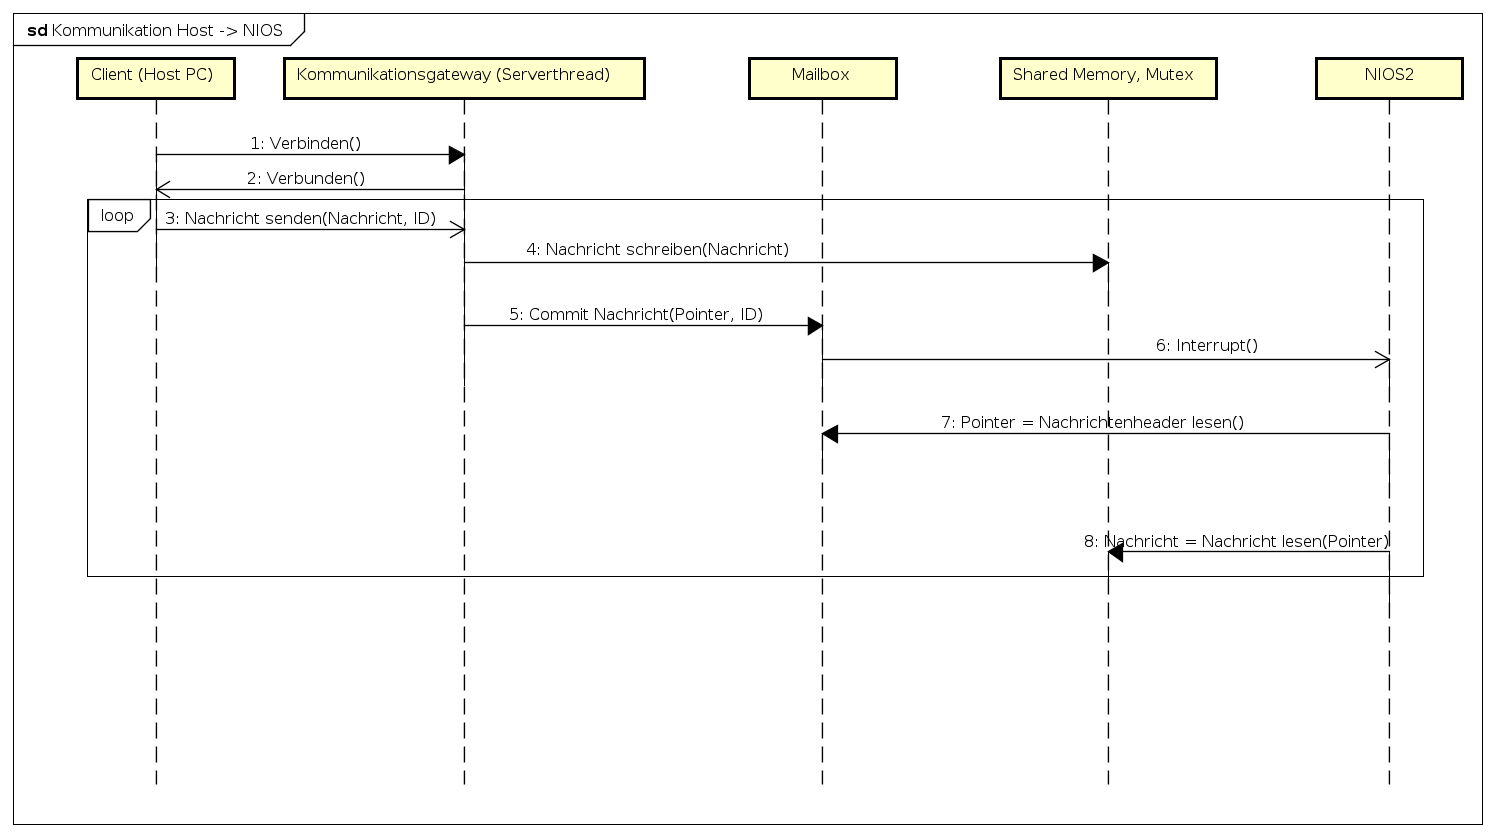
\includegraphics[width=\textwidth]{Abb/Komm_Host_NIOS.png}
	\caption{Kommunikationsablauf zwischen Host PC und NIOS}
	\label{SW:Komm:HOSTNIOS}
\end{figure}

\subsubsection{Empfohlener Buildvorgang und Abweichungen zum Tutorial}
Der schnellste und unkomplizierteste Weg zu einem funktionierenden Linux Image auf SD-Karte ist folgender
\begin{enumerate}
	\item Das Tutorial unter \href{https://eewiki.net/display/linuxonarm/DE0-Nano-SoC+Kit}{https://eewiki.net/display/linuxonarm/DE0-Nano-SoC+Kit} mit einer beliebigen (Mindestgröße 4GB) SD Karte durchführen. Als Kernelversion sollte unbedingt die Version 4.7 gewählt werden, da sich die im Projektrepository befindlichen Dateien darauf beziehen. Nach diesem Schritt kann man den Bootvorgang von U-Boot und Linux testen und versuchen sich im Ubuntu einzuloggen. Anschließend werden die Änderungen durchgeführt.
	\item Den Linux Devcie Tree Patchen. Dazu in einem Linux-Terminal
\lstset{language=bash}
	\begin{lstlisting}[breaklines=true]
patch socfpga-kernel-dev/KERNEL/arch/arm/boot/dts/socfpga_cyclone5_de0_sockit.dts socfpga_cyclone5_de0_sockit_garfield.patch #dieses Verzeichnis ist nach dem Tutorial verfuegbar
	\end{lstlisting}
	\item Das Linux Konfigurationsfile patchen
	\begin{lstlisting}[breaklines=true]
patch socfpga-kernel-dev/KERNEL/.config Garfield_Kernel.patch)
	\end{lstlisting}
	\item Anschließend über das Skript \texttt{socfpga-kernel-dev/tools/rebuild.sh} (oder manuell über den entsprechenden make-Befehl) den Kernel inkl. Device Tree neu kompilieren
	\item Den Linux Kernel und die Device Trees wie im Tutorial (die Punkte \texttt{Copy Kernel Image} und \texttt{Copy Kernel Device Tree Binaries}) auf die SD Karte kopieren.
\end{enumerate}

Anschließend kann man die SD-Karte wieder entnehmen und das \ac{FPGA} wieder einschalten. Das System sollte wie gewohnt starten. Um zu überprüfen, ob die Operationen funktioniert haben sollten folgenden Befehle die gleiche Ausgabe wie in Listing \todo{Verweis} haben. 
\todo{Listing einfügen, module uio und enable bridge enable}

\subsubsection{\ac{FPGA} Programmierung}
Die Programmierung des \ac{FPGA} Subsystems erfolgt unmittelbar während des Systemstarts und ist aktuell vom Softwarestart abgekoppelt. Das Image für das \ac{FPGA} wird dabei aus dem auf dem Board integrierten Flash-Speicher geladen. Die möglichen alternativen Konfigurationen sind übersichtlich im User-Manual zu dem \texttt{DE0-Nano} Board aufgelistet. Das Manual dazu findet man auf der System CD, die unter \href{http://www.terasic.com/downloads/cd-rom/de0-nano-soc/}{Link} verfügbar ist.\\

Auf dem Flash befindet sich sowohl das Image für das \ac{FPGA} als auch das executable für den nach dem flashen im \ac{FPGA} verfügbaren NIOS2. \todo{Kopie?}
\subsubsection{Applikationsstart}
Für die Kommunikation zwischen Host PC und NIOS2 ist das starten des Kommunikationsgateway erforderlich. Dies befindet sich unter \texttt{HPS/bin/Comm\_Gateway} und ist das Kompilat des oben beschriebenen \todo{Name}. Damit das Programm Ordnungsgemäß funktionieren kann müssen noch einige Schritte durchgeführt werden, die hier kurz erklärt werden.

\lstset{language=bash}
\begin{lstlisting}[caption=Listing, label={StartApp}]
	sudo -s # superuserrechte erlangen, Passwort = temppwd
	rmmod uio_pdrv_genirq
	rmmod uio
	modprobe 
	ls /dev/
	bin/Comm_Gateway
\end{lstlisting}

Der Codeausschnit \ref{StartApp} zeigt alle durchzuführenden Schritte, die notwendig sind um das Kommunikationsgatway ordnungsgemäß zu starten. Die ersten beide Befehle entfernen evtl. geladenene Module, die beim startup mit falschen Parametern geladen werden. Der dritte Befehl lädt das Linux-Modul um mit Interrupts im User-Space umgehen zu können und erstellt dafür ein Gerät mit dem Namen \texttt{HSP\_boot/dev/uio0}, dass im Kommunikationsgatway verwendet werden. Hier ist auch der Name, der im Linux Device Tree angegeben wurde, von Bedeutung, da über diesen das richtige Interrupt ausgewählt wird. Mit dem vierten Befehl sollte vor Ausführung des Gateways überprüft werden ob das Gerät \texttt{HSP\_boot/dev/uio0} auch wirklich verfügbar ist. Ist dies der Fall, kann die Applikation mit Superuserrechten gestartet werden. Die Reihenfolge ist dabei
\begin{enumerate}
	\item Starten des FreeRTOS auf dem NIOS2 (wird i.d.R. automatisch bei Systemstart durch Laden aus dem externen Flash durchgeführt).
	\item Konfigurieren des Linux und starten der Applikation (eine Serververbindung wird angeboten).
	\item Anschließendes Verbinden der Applikation auf dem Host-PC mit dem Server. Daten werden ab diesem Zeitpunkt ausgetauscht.
\end{enumerate}

\subsubsection{Beenden der Applikation}
Aktuell ist keinerlei Fehlerbehandlung für das Beenden der Client-Server Verbindung (Host-PC $\leftrightarrow$ \ac{HPS}) vorhanden. Beendet der Client die Kommunikation hängt sich das gesamte System auf (Grund: Interrupts werden nicht mehr angenommen und der interne Bus wird durch die Mailbox blockiert!). Es ist also unbedingt notwendig die Applikation auf dem laufenden Linux mittels eines \lstinline|SIGINT| (STRG+C) zu beenden. Alternativ kann man dem Programm auch auf der Kommandozeile oder durch z.B. htop das Signal schicken. Mit dem Signal sendet Linux einen speziellen Befehl an den NIOS2 wodurch dieser die Kommunikation auch beendet. Werden wieder Befehle geschickt, wird die Kommunikation von beiden Seiten wieder aufgenommen.
 


\section{$\mu$Controller - NIOS2}
 \chapter{Operating System - FreeRTOS}
 Dieses Kapitel beschreibt die Benutzung des verwendeten Betriebssystemes, das FreeRTOS. 
 \section{Tasks}
 \begin{itemize}
  \item Scheduler
  \item Erzeugung
  \item Zyklisch aufrufen
 \end{itemize}

 \section{RTOS Config}
 Hier wird die genaue RTOS Konfiguration beschrieben, die benutzt wurde für das OS auf dem NIOS2.
 \section{benutzte Tasks}
 Hier werden dann die tatsächlich benutzten Task erläutert, die auf dem NIOS2 laufen und für alle wichtigen Aufgaben zuständig sind.


\chapter{NIOS2 - HAL}
Hier wird kurz der Aufbau der HAL bzw. der Aufbau der jetzt zur Verfügung stehenden Treiber des NIOS2 Cores erläutert. Genauere Dokumentation ist in der Doxygen Dokumentation zu finden, die im Anhang mitgeliefert wird. 
\section{Display}
Das Display kann sogar Zahlen anzeigen
\section{Motor}
Die Ansteuerung des Motors passiert folgendermaßen: ...
\section{Lenkung}
Lenken geht auch
\section{MPU6050}
Das mpu6050 Modul ist über den IIC Bus angeschlossen und kann viele tolle Sachen.
\section{Ultraschall}
Die vier zur Verfügung stehenden Ultraschallsensoren sind über den gleichen IIC Bus, wie das MPU6050 Modul angebunden. 


 \chapter{Operating System - FreeRTOS}
 Dieses Kapitel beschreibt die Benutzung des verwendeten Betriebssystemes, das FreeRTOS. 
 \section{Tasks}
 \begin{itemize}
  \item Scheduler
  \item Erzeugung
  \item Zyklisch aufrufen
 \end{itemize}

 \section{RTOS Config}
 Hier wird die genaue RTOS Konfiguration beschrieben, die benutzt wurde für das OS auf dem NIOS2.
 \section{benutzte Tasks}
 Hier werden dann die tatsächlich benutzten Task erläutert, die auf dem NIOS2 laufen und für alle wichtigen Aufgaben zuständig sind.

\subsection{Eclipse NIOS2}
\subsubsection{C++ - Beschränkungen, besondere Einstellungen}
Das in der 16.1 verwendeten Quartus mit dem mitgeliefertem GCC Compiler hat einige Einschränkungen bezüglich der Verwendung von einigen C++ Features. Alle in den C++ Standardbibliotheken vorhandenen STL Container, z. B. std::vector, std::stack, std::map usw., sind nicht benutzbar. Außerdem ist es nicht möglich die std::string Klasse zu benutzen. Die Benutzung solcher Features führt dazu, dass der Speicher nicht mehr ausreicht. Für die Verwendung dieser Klassen sind auf dem NIOS2 mit der aktuellen Toolchain ca 700KB RAM nötig, allerdings sind nur 128KB RAM vorhanden. Dies wurde vom ALTERA Support Team direkt bestätigt mit der Angabe, dass die Benutzung von C++ im Moment nicht effizient möglich ist und externer Speicher für die Verwendung von C++ angeraten ist. Alle anderen Features hingegen sind, soweit bekannt, ohne Einschränkungen benutzbar.

Für die Unterstützung von c++11 ist eine kleine manuelle Anpassung des Makefiles nötig, welches die Toolchain mit Erstellung eines BSP automatisch generiert. In der Sektion
\begin{itemize}
 \item \# Arguments only for the C++ compiler.
\end{itemize}
ist die Ergänzung folgenden Flags nötig: -std=c++11; da diese Einstellung über die GUI nicht erhalten bleibt. Die Sektion sollte dann folgendermaßen aussehen:
\begin{itemize}
 \item \# Arguments only for the C++ compiler.\\APP\_CXXFLAGS := \$(ALT\_CXXFLAGS) \$(CXXFLAGS) \ \\-std=c++11
\end{itemize}
Diese Einstellung ist auch unbedingt nötig, da einige c++11 Features verwendet wurden und demzufolge ohne diesem Flag die Applikation nicht erfolgreich kompiliert.

\subsubsection{Die externen/internen ips}
Qsys bemühen, die mitzunehmen, sonst fehlt da was; siehe git doku?


\chapter{NIOS2 - HAL}
Hier wird kurz der Aufbau der HAL bzw. der Aufbau der jetzt zur Verfügung stehenden Treiber des NIOS2 Cores erläutert. Genauere Dokumentation ist in der Doxygen Dokumentation zu finden, die im Anhang mitgeliefert wird. 
\section{Display}
Das Display kann sogar Zahlen anzeigen
\section{Motor}
Die Ansteuerung des Motors passiert folgendermaßen: ...
\section{Lenkung}
Lenken geht auch
\section{MPU6050}
Das mpu6050 Modul ist über den IIC Bus angeschlossen und kann viele tolle Sachen.
\section{Ultraschall}
Die vier zur Verfügung stehenden Ultraschallsensoren sind über den gleichen IIC Bus, wie das MPU6050 Modul angebunden. 


\chapter{Zusammenfassung}
Im Rahmen dieses HSP Projekts konnten die anfangs gesteckten Ziele weitgehend erreicht werden. Durch Ersetzen des Raspberry Pi durch eine flexible (FPGA) und leistungsstarke (ARM A9 Dualcore) Lösung, wurde eine Möglichkeit geschaffen sowohl Echtzeitbedingungen als auch low level IO Operationen (I2C, SPI, PWM etc.) von dem Hauptprozessoren zu entfernen. Durch diesen Schritt sind auf dem Hauptprozessor genug Leisutungsreserven frei um in zukünftigen Anwendungen Berechnungen, wie z.B. zur Berechnung von SLAM Algorithmen, direkt auf den Hauptprozessoren durchzuführen. Gleichzeitig hat das FPGA noch genug freie Logik zur Verfügung, um Teile von SLAM Algorithmen u.U. direkt auf Hardware rechnen zu können. Gleichzeitig konnten alle Funktionalitäten der Ausgangsbasis erhalten werden, wodurch dieses Projekt eine gute Grundlage für die Bearbeitung durch weitere Gruppen bildet.

\section{Schaltplan}

\begin{figure}
	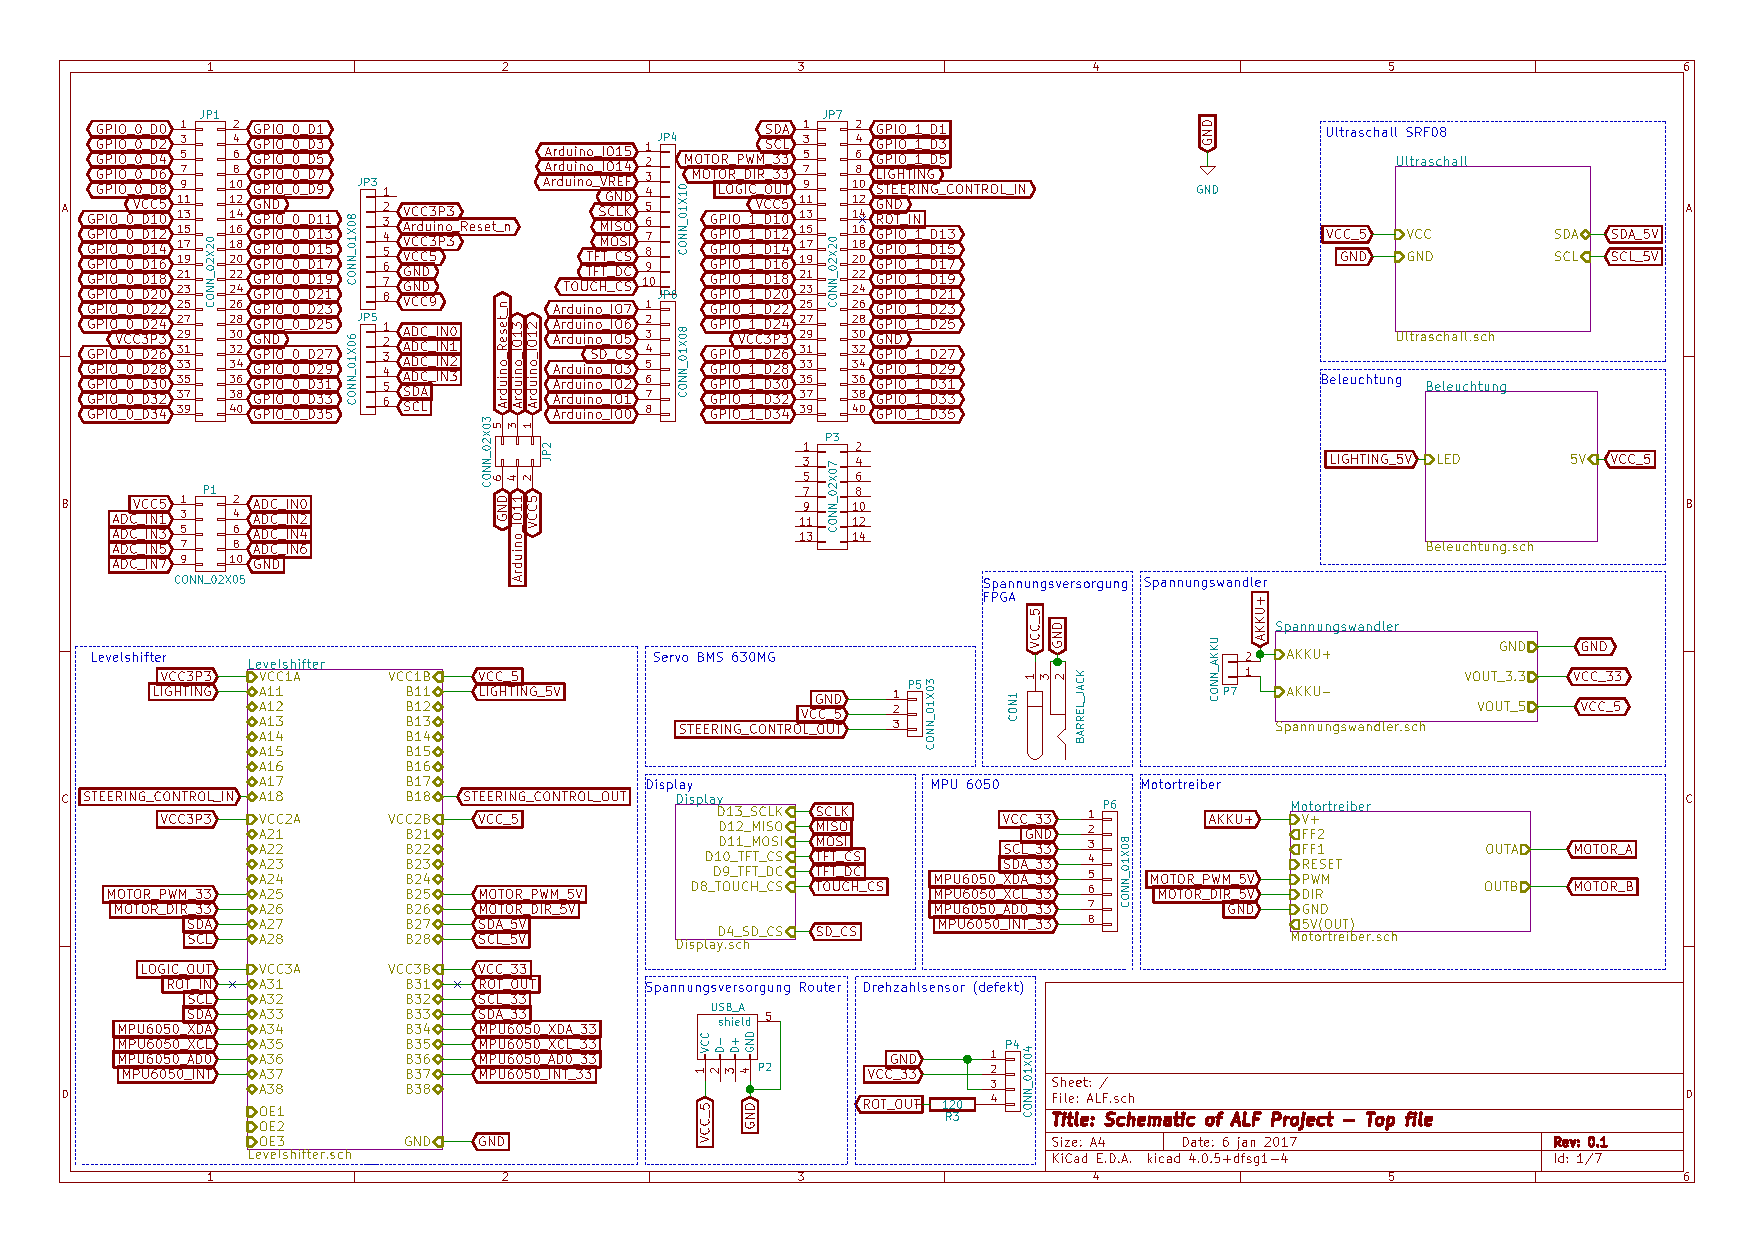
\includegraphics[angle=90, height=\textheight]{Abb/Garfield_Circuit.pdf}
	\caption{Schaltplan mit FPGA und verwendeter Peripherie}
	\label{Garfield_Circuit}
\end{figure}
Abbildung \ref{Garfield_Circuit} zeigt den erstellten Schaltplan des HSP. Dieser soll nachfolgend kurz beschrieben werden.\\
Alle ein- und ausgeheneden Signale mit Ausnahme der SPI Pins zur Ansteuerung des Displays (vgl. Abb. \ref{Garfield_Circuit} JP4) werden über Levelshifter geführt. Dies ermöglicht es zum einen alle Signale an die jeweils notwendigen Pegel anzupassen und zum anderen den maximalen vom FPGA bereitgestellten Strom nicht zu überschreiten. Dadurch ergeben sich die zwei Logikpegel 3,3V und 5V im System. Über den IIC Port werden alle Ultraschallsensoren und die MPU6050 angesprochen. Es wurden die internen pull-up Widerstände des IIC Ports aktiviert um dessen Funktionsfähigkeit sicherzustellen. Über den PWM Generator wird die Lenkung und der Motortreiber für die Geradeausfahrt angesteuert. Zur Ansteuerung der Beleuchtung und dem Setzen der Richtung des Motors werden einfache GPIO Pins benutzt. Der Schaltplan enthält zudem die Ansteuerung des Rotary Encoders zum Messen der Drehzahl des Motors. Da dieser jedoch unerwarteterweise nicht funktionsfähig war, sind die betrefenden Stellen im Schaltplan entsprechend gekennzeichnet.
\section{\ac{FPGA} Design}
Die Beschreibung des \ac{FPGA} wird, soweit möglich, mit dem Systemintegrationstool QSYS, das Teil der Quartus Toolchain ist, durchgeführt. Das Mapping zwischen QSYS-System und Pins wird klassisch in VHDL beschrieben. Das Top-Level-File des Systems ist \\ \texttt{FPGA\_Design/Garfield\_Design/Garfield.vhdl}. Dort wird das von QSYS erzeugt System und einige kleine \ac{IP}-Cores zusammengeführt und auf definierte Aus-/Eingänge geführt. Diese Ein-/Ausgänge werden dann über den \textit{Pin-Planner} auf die physikalischen Pins geführt.\\
Im Projektverzeichnis befinden sich alle Dateien, die für den \ac{FPGA} Teil relevant sind, unter \texttt{FPGA\_Design}. Die Struktur ab diesem Ordner ist wie folgt aufgebaut:
\begin{itemize}
	\item \texttt{Datasheets} - Einie Datenblätter und Application Notes zu dem \ac{FPGA} Teilprojekt
	\item \texttt{Garfield\_Design} - In diesem Ordner befinden sich die Quartus Projektdateien, Konfigurationsdateien und das QSYS Projekt.
	\item \texttt{ip\_extern} - Eine Sammlung von externen \ac{IP}-Cores, die im Projekt verwendet wurden. Es befinden sich dort nur die \ac{IP}-Cores, die nicht von Altera stammen oder nicht direkt in QSYS verfügbar sind.
	\item \texttt{ip\_intern} - Alle \ac{IP}-Cores, die für dieses Projekt entwickelt wurden.
	\item \texttt{output\_files} - In jedem Unterordner innerhalb dieses Ordners befinden sich \ac{FPGA} Images und die entsprechenden Konfigurationsdateien um ein Softwareprojekt dafür zu bauen.
\end{itemize}

Im folgenden werden die alle Systemkomponenten, die für das \Projectname-Projekt erzeugt wurden, beschrieben.

\section{\ac{IP}-Cores}
\label{IP-Cores}

\begin{figure}
	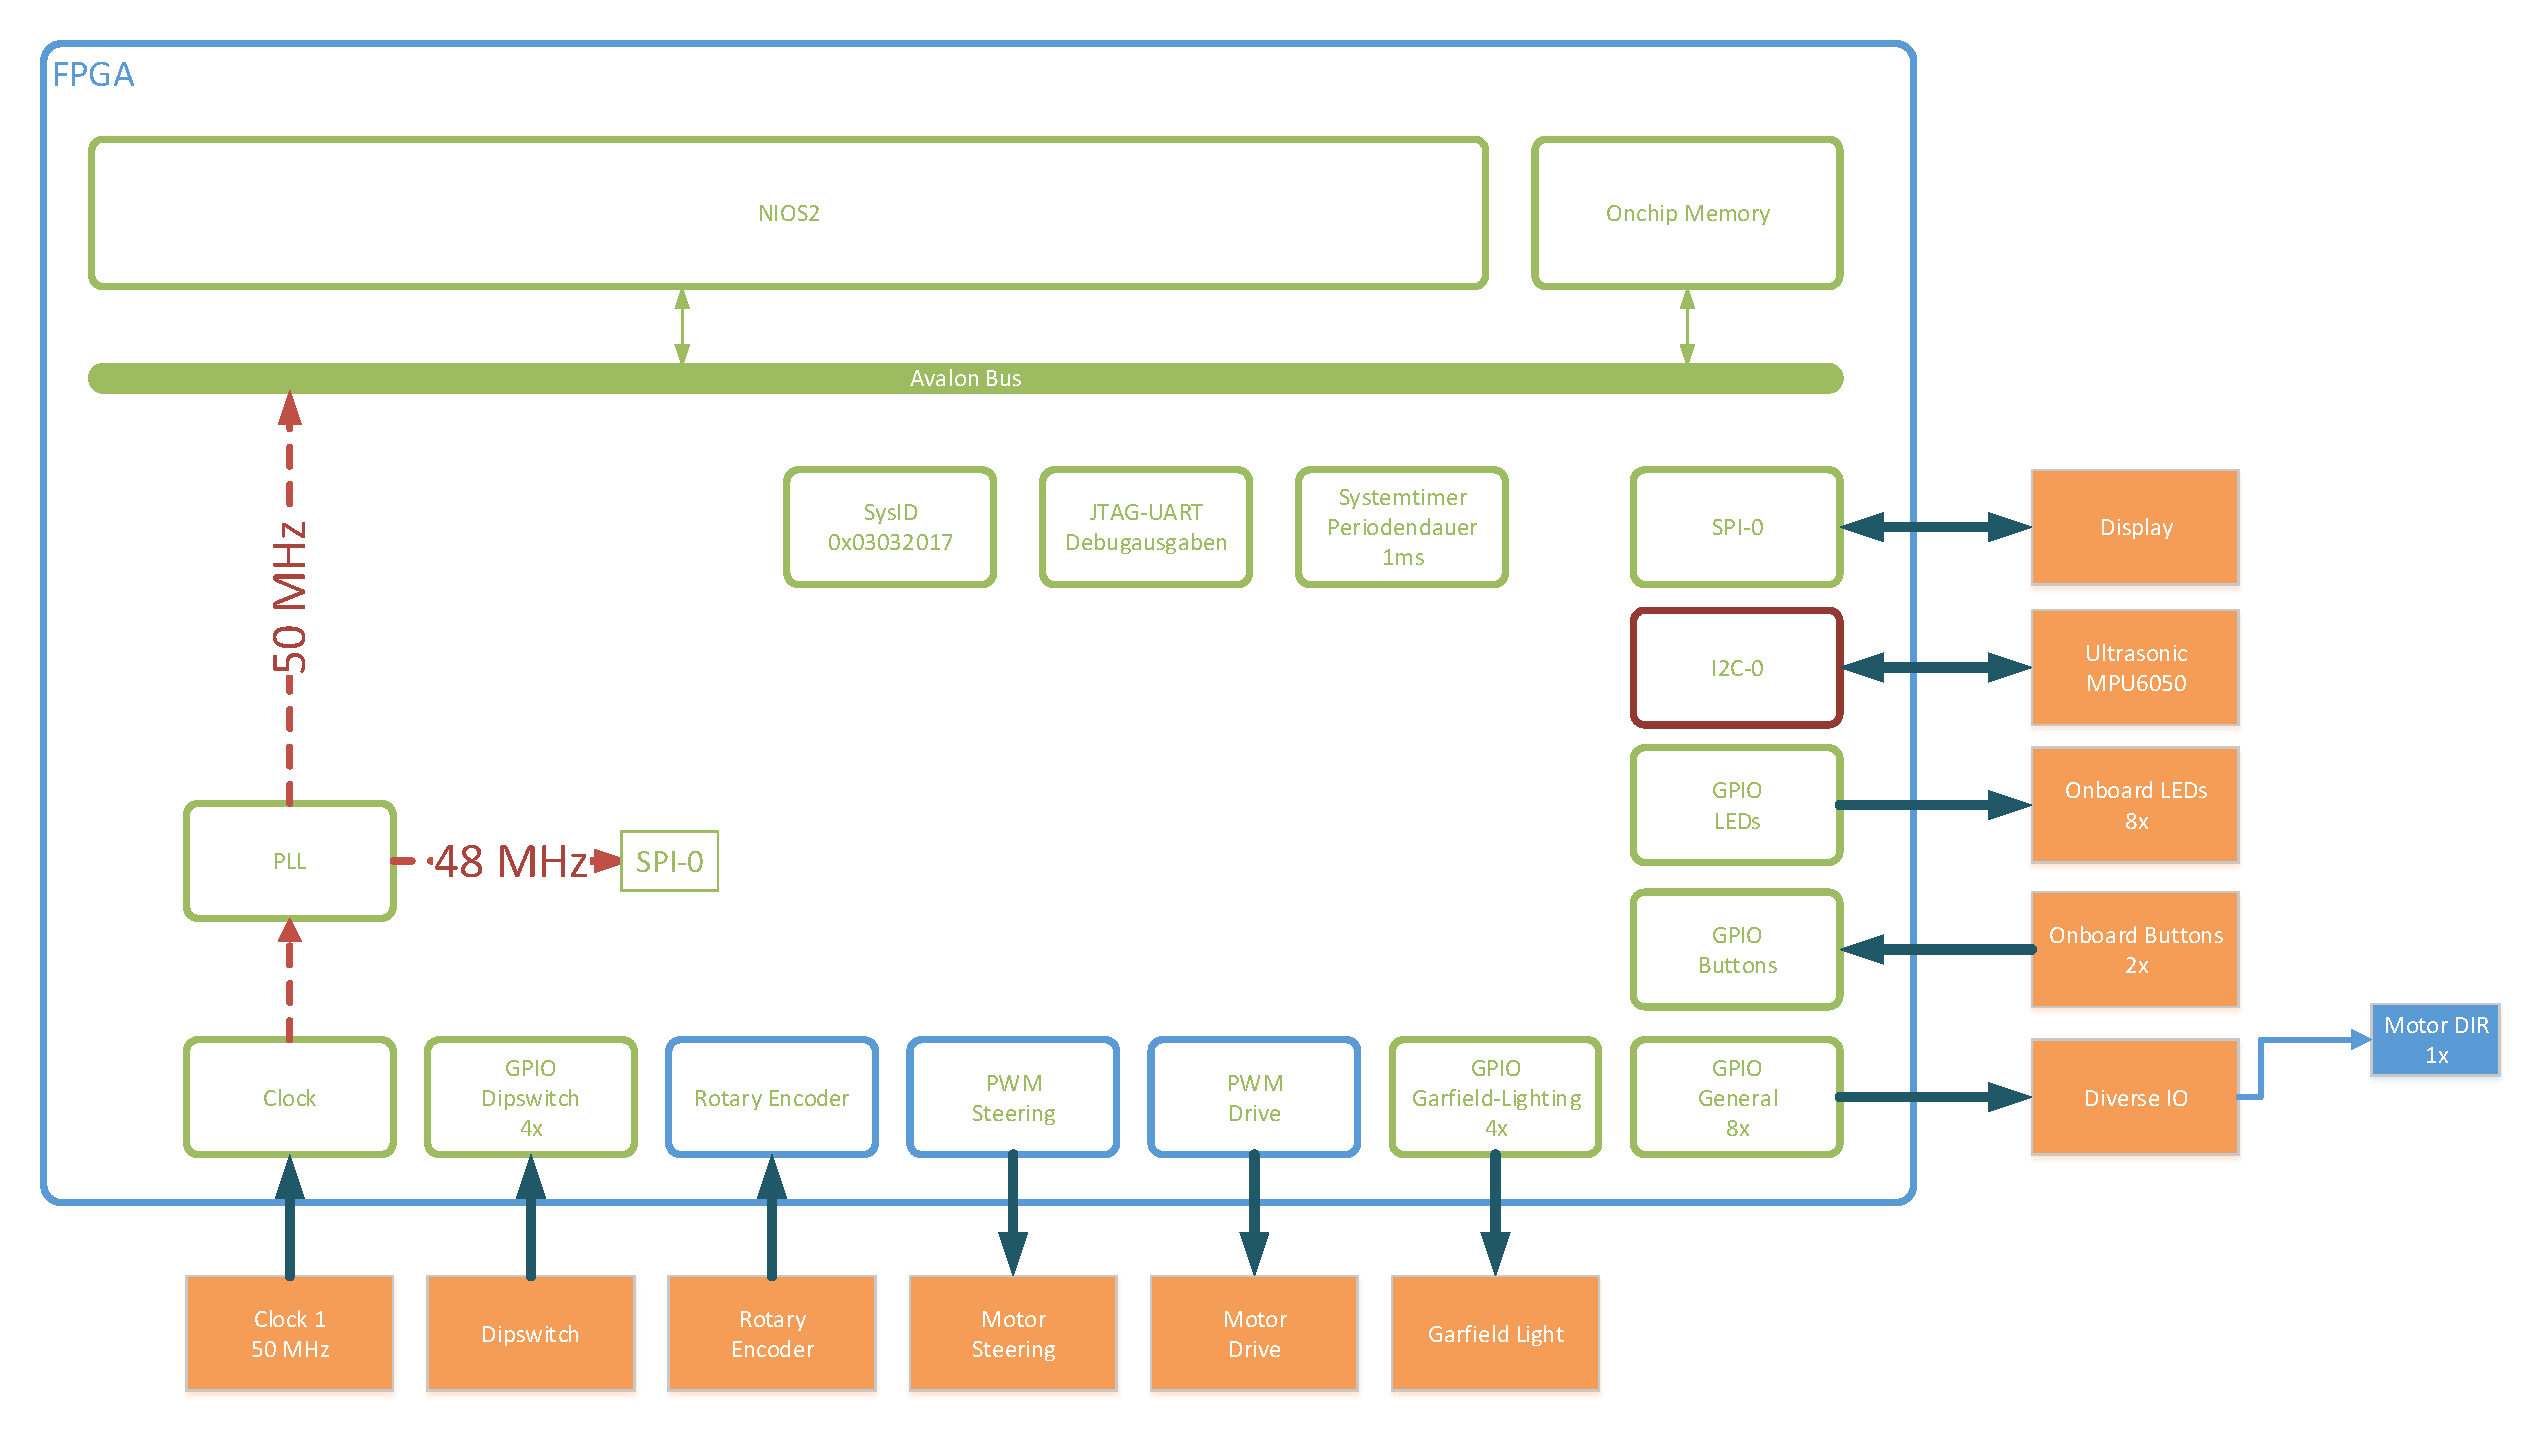
\includegraphics[angle=90, height=0.9\textheight]{Abb/Garfield_FPGA_Design_only_FPGA.pdf}
	\caption{Übersicht der (meisten) eingesetzten \ac{IP}-Cores. Die Abbildung verzichtet auf die Darstellung der Teile, die für die Kommunikation mit dem \ac{HPS} zuständig sind. Blau umrandet sind Cores, die im Rahmen des Projekts selbst progammiert wurden, grün diejenigen, die Teil der Altera Toolchain sind und rot externe IP-Cores von opencores.org}
	\label{FPGA_IP_FPGA_only}
\end{figure}

Abbildung \ref{FPGA_IP_FPGA_only} zeigt eine Übersicht der eingesetzten \ac{IP}-Cores und deren Verbindung zur Außenwelt. Ausgenommen sind die \ac{IP}-Cores, die für die Kommunikation mit dem \ac{HPS} benötigt werden. Die nachfolgende Tabelle beschreibt die Funktion der einzelnen IP-Cores im Detail und Besonderheiten dazu.

\begin{longtable}[ht]{|p{0.1\textwidth} | p{0.9\textwidth} |}
	\hline
	\textbf{Name} & \textbf{Beschreibung}\\
	\hline
	SPI-0 & Stellt einen SPI-Datenbus mit 24MHz Clock-Frequenz zur Verfügung. Es werden insgesamt 3 Chipselect Signale zur Verfügung gestellt, wobei aktuell nur eines für das Display benutzt wird. In der aktuellen Ausbaustufe wird nur das Display auf dem Arduino-Header auf dem FPGA angesteuert.\\ \hline
	I2C-0 & Stellt einen I2C Datenbus zur Verfügung. Der \ac{IP}-Core stammt von \href{opencores.org}{opencores.org} und wurde manuell integriert. Er stellt u.a. eine eine in Software änderbare Clock-Frequenz zur Verfügung und bindet die Ultraschallsensoren und die MPU-6050 an das System an.\\ \hline
	GPIO-X & Die verschiedenen GPIO Cores dienen dazu einfache Peripherie anzubinden. Dazu gehören die LEDs, die Dip-Switches, die Buttons und generische IOs, die im Projekt benötigt werden um z.B. die Drehrichtung des Motors einzustellen. \\ \hline
	PWM X & Die beiden PWM \ac{IP}-Cores erzeugen Signale zur Geschwindigkeitssteuerung und für den Lenkmotor. \\ \hline
	Rotary-Encoder & Der Rotary Encoder zählt die steigenden Flanken der NAME. Durch Abfragen des Ergebnisregisters in regelmäßigen festen Zeitinervallen kann die aktuelle Geschwindigkeit, die an den Rädern anliegt, gemessen werden. Leider funktioniert der NAME aktuell nicht mehr. Um das Signal zu nutzen müsste man die Hardware neu aufbauen bzw. ersetzen.\\ \hline
	Clock \& \ac{PLL} & Die externe Referenzclock taktet mit 50 MHz. Dieses Signal wird über eine \ac{PLL} allen beteiligten IP-Cores bereitgestellt. Auch die \ac{FPGA}-\ac{HPS} Bridges werden mit dem 50MHz Signal gespeist. Einzige Ausnahme bildet der SPI-0 Core. Um eine Frequenz von 24MHz zu erreichen (die maximale Frequenz mit der das Display angesprochen werden darf) wird ein vielfaches dieser Frequenz benötigt. Das nächsthöhere verfügbare vielfache der 24MHz sind 48MHz. Die selbst geschriebenen \ac{IP}-Cores sind von der Frequenz der \ac{PLL} abhängig. Erhöht man die Frequenz der \ac{PLL} auf z.B. 100MHz um mehr Laufzeit für einzelne Funktionen zur Verfügung zu haben, muss man die Frequenz in den \ac{IP}-Cores manuell anpassen! \\ \hline
	SysID & Mit der System ID (in Kombination mit einem Zeitstempel) kann man das Hardware Design eindeutig identifizieren. Dies ist hilfreich wenn mehrere Hardware- und Softwareversionen existieren, die parallel entwickelt werden. Um Zugriffsfehler auf Register oder ähnliches zu vermeiden, kann die Software die System-ID nutzen um Funktionen ab- bzw. zuzuschalten. \\ \hline
	JTAG-UART & Mit Hilfe dieses Cores kann man printf ähnliche Ausgaben für Debug-Ausgaben an einen angesteckten PC schicken. \\ \hline
	Systemtimer & Der Systemtimer ist ein kontinuierlich laufender Timer, der sich alle 1ms automatisch erhöht. Außerdem erzeugt er ein Interrupt, das FreeRTOS zur internen Zeitbestimmung nutzt. \\ \hline
	NIOS2 & Hierbei handelt es sich um eine Softcore-CPU. Diese wird von Altera zur Verfügung gestellt (inkl. Toolchain) und kann unbegrenzt benutzt werden (mit entsprechender Lizenz). Es handelt sich um eine 32-bit \ac{RISC} Architektur die durchaus eine weite Verbreitung im industriellen Umfeld genießt. Weiter Informationen dazu findet man unter \href{https://www.altera.com/products/processors/overview.html}{https://www.altera.com/products/processors/overview.html} \\ \hline
	Onchip Memory & Ein einfacher \ac{IP}-Core, der Speicherbausteine auf dem \ac{FPGA} nutzt um RAM(hier genutzt) oder ROM (nicht genutzt) zu erzeugen. Dieser Speicher kann dann von einem Prozessor (hier der NIOS2) als Instruktions- und Datenspeicher genutzt werden. In der aktuellen Ausbaustufe ist die Speichergröße mit 128kB angegeben. \\ \hline
\end{longtable}
\todo{NAME}

\begin{figure}
	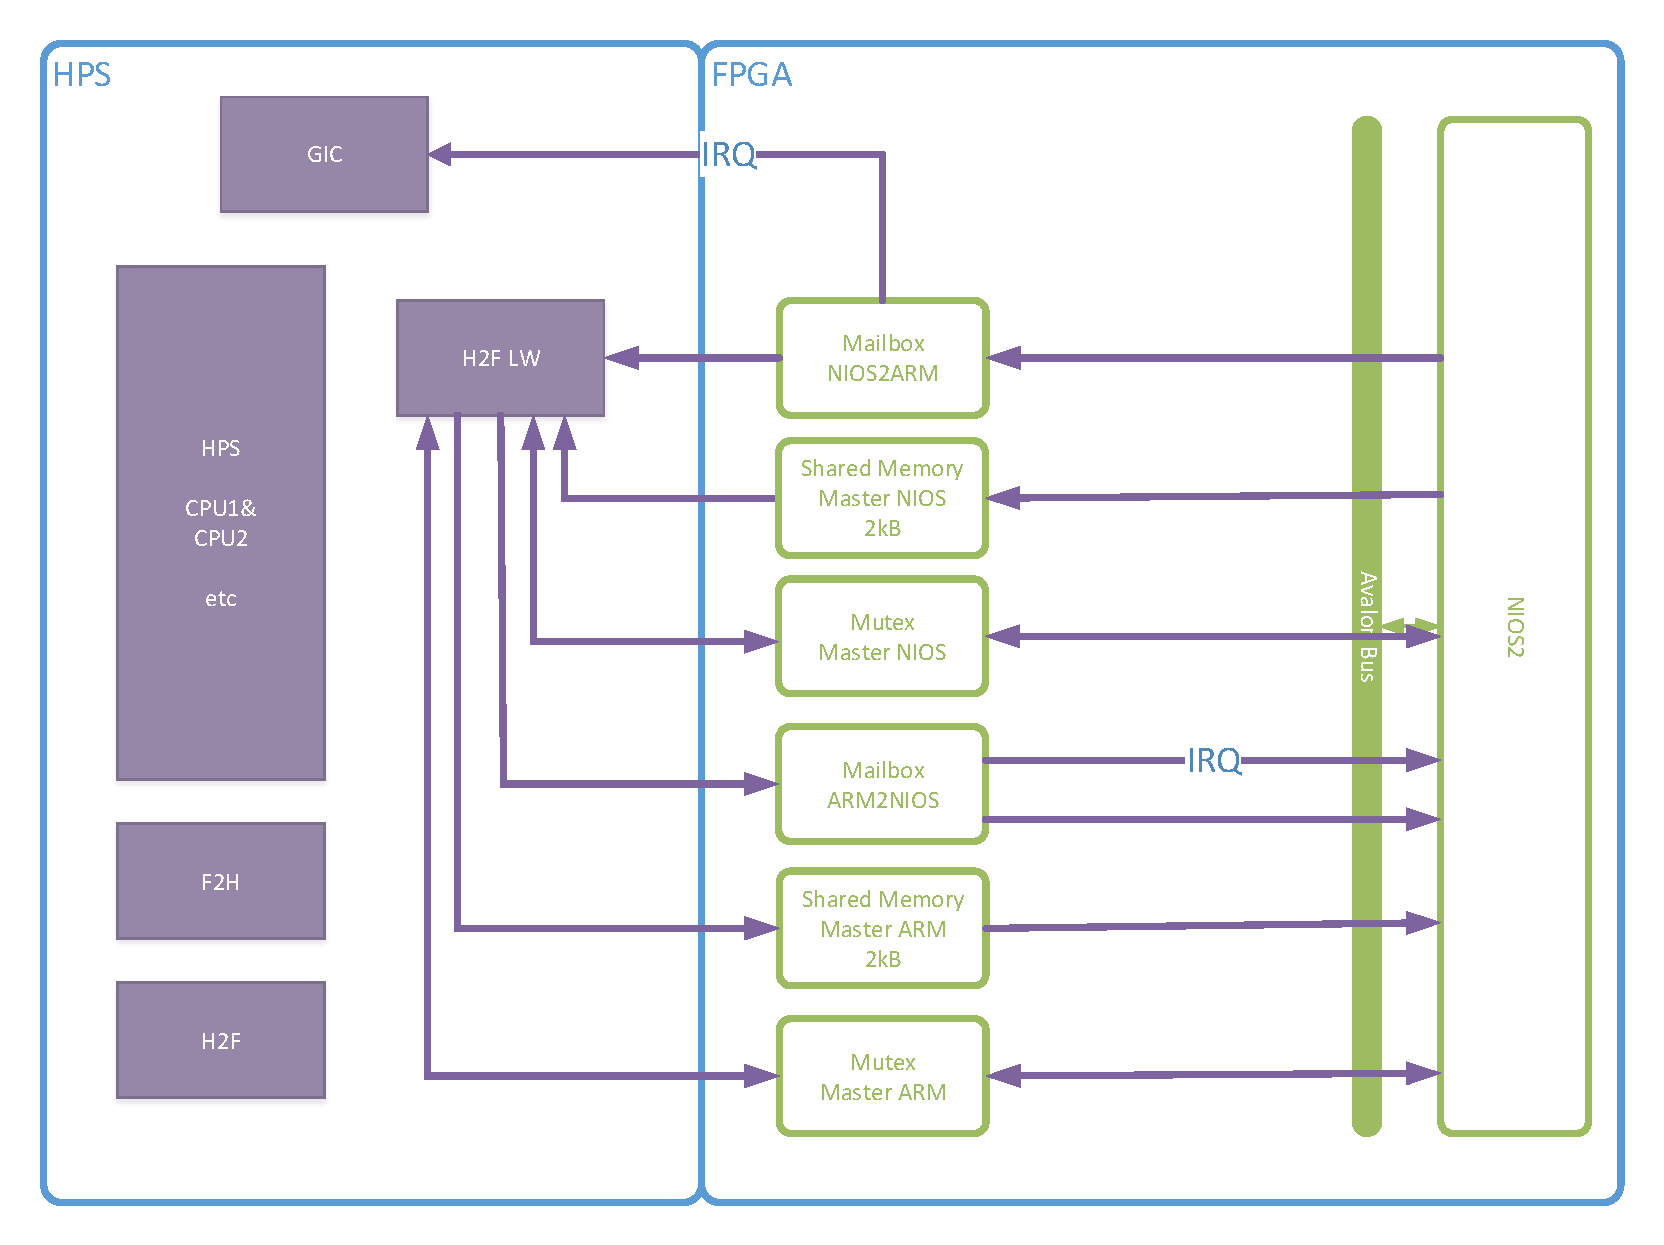
\includegraphics[angle=0, width=\textwidth]{Abb/Garfield_FPGA_Design_comm.pdf}
	\caption{\ac{IP}-Cores und deren Kontrollfluss, die an der Kommunikation zwischen NIOS2 und \ac{HPS} beteiligt sind.}
	\label{FPGA_IP_FPGA_comm}
\end{figure}

Abbildung \ref{FPGA_IP_FPGA_comm} zeigt die \ac{IP}-Cores, die für die Kommunikation zwischen \ac{FPGA} und \ac{HPS} benötigt/eingesetzt werden. Auf der linken Seite der Abbildung ist das \ac{HPS} System illustriert. Auf dieser Seite sind im wesentlichen drei Hardwareeinheiten an der Kommunikation beteiligt:
\begin{itemize}
	\item GIC - Der ARM \textit{General Interrupt Controller} : Dieser Controller ist ein sehr mächtiger Interrupt Controller, der u.a. die Interruptverarbeitung an die einzelnen CPUs verteilt. Insgesamt stehen 64 Interrupts zur Verfügung, die aus dem \ac{FPGA} heraus ausgelöst werden können. Auf dem eingesetzten Cyclone V beginnen diese mit der Interrupt ID 72 vom GIC. Genauere Informationen zum GIC kann man entweder auf der Homepage von ARM oder \cite{Using_GIC} erhalten.
	\item H2F LW - Die \ac{HPS}2\ac{FPGA} Leightweight Bridge : Dies ist eine der drei Bridges, mit denen zwischen \ac{FPGA} und \ac{HPS} kommuniziert werden kann. Dies ist keine High-Performance Bridge, es ist aber keine großen Änderungen notwendig, das System auf eine der anderen Bridges umzubauen. Diese Bridge \textbf{muss} aktiviert werden, bevor über sie kommuniziert werden kann. Ist die Bridge nicht aktiviert, treten \textit{Segmentation Faults} auf (kein gültiger Speicherbereich). Im Prinzip befindet sich \textquotedblleft hinter\textquotedblright der Bridge ein Speicherbereich, der durchgehend addressiert werden kann um direkt in Register zu schreiben. Auch lesende Zugriffe daraus können erfolgen \cite{FPGA_Workshop}.
	\item CPUs - Die ARM A9 Applikationsprozessoren dienen zur Verarbeitung der Interrupts bzw. zum triggern der einzelnen IP-Cores.
\end{itemize}

Es folgt eine Beschreibung der \ac{IP}-Cores, die für die Kommunikation gebraucht werden. Da die Kommunikationseinheiten in beide Richtungen analog aufgebaut sind, beschränkt sich die Beschreibung auf einen Richtung:
\begin{itemize}
	\item Mailbox X2Y : Die Mailbox ist ein einfacher IP-Core der Nachrichten von einem Buspartner (X, z.B. NIOS2) einem anderen Buspartner (Y, z.B. ARM) zur Verfügung stellt. Es gibt also einen Transmitter und einen Receiver. Beide sind über eigene Interfaces (und damit über ihren eigenen Addressbereich) an die Mailbox angeschlossen. Die Nachrichtenübermittlung erfolgt mit Hilfe von zwei Registern:
	\begin{itemize}
		\item Command Register - Dieses Register kann vom Empfänger nur gelesen werden. Es dient dazu, ein Kommando oder Nachricht an den Empfänger zu senden. Ein schreibender Zugriff auf dieses Register vom Sender löst das zugehörige Interrupt aus, dass vom Empfänger verarbeitet werden muss.
		\item Pointer Register - In diesem Register wird die Addresse, in der die eigentliche Nachricht im Speicher steht, übertragen. Sollen nur ganz kleine Nachrichten (4 oder 8 Bytes) übertragen werden, kann man das Pointer und Command Register dazu benutzen, die Nachricht zu übertragen. In diesem Projekt wird aber die eigentliche Nachricht im Shared Memory übertragen, in der Mailbox nur die Addresse im Shared Memory und ein Kommando im Command Register
	\end{itemize}
	Eine detailierte Beschreibung des Cores findet sich unter \cite[470ff]{embedded_guide}
	\item Shared Memory Master X - Dieser Speicher, der wie der Arbeitsspeicher des NIOS2 direkt im \ac{FPGA} synthetisiert wird, dient der Nachrichtenübermittlung. Dort werden die Nutzdaten einer Nachricht von X reingeschrieben und können zu einem späteren Zeitpunkt vom Empfänger Y ausgelesen werden. Es wurde sich bewusst dazu entschieden zwei Shared Memory zu benutzen um eine jegliche Kollision zu vermeiden bzw. zu vereinfachen. Die Größe beider Speicherbereiche beträgt jeweils 2kB. Dies reicht für die aktuellen Nachrichten leicht aus. Zu einem späteren Zeitpunkt können die Bereiche auch noch vergrößert werden, sollte der Speicher nicht groß genug sein Nachrichten zu übertragen.
	\item Mutex Master X - Dies ist ein spezieller \ac{IP}-Core, der auch als Teil des Altera \ac{IP}-Core Katalogs zur Verfügung stellt. Dieser hat nur ein Register, das hier betrachtet werden soll und erlaubt einen atomaren Mutex Zugriff auf geteilte Resourcen. Die geteilte Resource, die über diesen Mutex gesperrt wird ist der zugehöriger Shared-Memory. Die Referenz für diesen Core ist ebenfalls \cite[319ff]{embedded_guide}. Das Register besteht aus zwei Teilen: die oberen 16 Bit werden als Speicherplatz für die CPU-ID (der NIOS2 hat die ID 0x03, der ARM immer 0x01) benutzt. In die unteren 16 Bit kann ein beliebiger Wert gespeichert werden. Ein lesender Zugriff auf den Mutex ist immer möglich. Ein schreibender Zugrif ist nur möglich wenn
	\begin{itemize}
		\item Die CPU-ID mit der CPU-ID übereinstimmt, dessen Wert man in das Register schreiben will.
		\item (oder) Der Wert (untere 16-Bit) Null ist.
	\end{itemize}
	Man kann also nur schreibend auf den Mutex zugreifen, wenn einem der Mutex bereits gehört oder der Mutex frei (=0) ist. Nach einem schreibenden Zugriff muss der Registerwert mit dem Wert der geschrieben wurde verglichen werden. Stimmen beide Werte überein, hat der Schreiber den Mutex gelockt, andernfalls ist der atomare Lock fehlgeschlagen.
\end{itemize}

\section{Address-Map}

\begin{figure}
	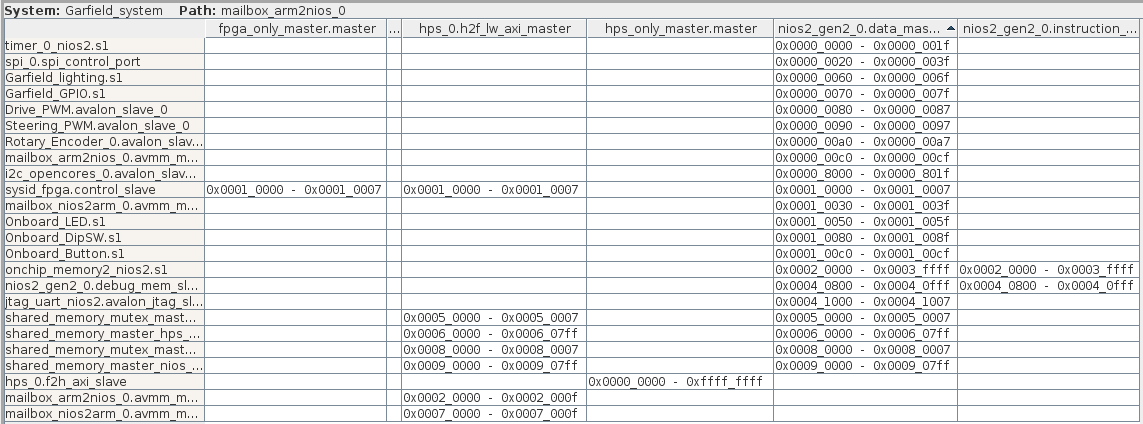
\includegraphics[width=\textwidth]{Abb/Address_Map.png}
	\caption{Übersicht über die Addressen und Addressbereiche im System}
	\label{FPGA:AddrMap}
\end{figure}

Abbildung \ref{FPGA:AddrMap} zeigt die Addressen die im System benutzt werden und den zugehörigen Addressbereich der verfügbar ist. Diese Addressmap ist auch im QSYS-Projekt des Projektes verfügbar.

\section{Eigenentwickelte \ac{IP}-Cores}

\subsection{Der PWM-Generator} generiert ein PWM Signal auf die Ausgabeleitung. Der Registerzugriff ist in Tabelle \ref{hw:pwm} dargestellt

\begin{table}
\begin{longtable}[]{@{}c|l|c|c|l@{}}
	\textbf{Bit} & \textbf{Name} & \textbf{Access} & \textbf{Reset Value} &
	\textbf{Description}\tabularnewline

	\endhead
	\texttt{7\ ...\ 0} & control & RW & 0 & sets the dutycylce of the PWM
	signal generator\tabularnewline
	\texttt{31\ ...\ 7} & - & R & 0 & not used\tabularnewline

\end{longtable}
\caption{Registermap des PWM Cores}
\label{hw:pwm}
\end{table}

\subsection{Der Rotary Encoder} \ac{IP}-Core kann steigende Flanken von einer externen Flanke zählen, hat ein auslesbares Ergebnisregister (siehe \ref{hw:rotary:result})und ein Controlregister (siehe \ref{hw:rotary:control}).

\begin{table}
\begin{longtable}[]{@{}clccl@{}}
	\begin{minipage}[b]{0.13\columnwidth}\centering\strut
		\textbf{Bit}\strut
		\end{minipage} & \begin{minipage}[b]{0.08\columnwidth}\raggedright\strut
		\textbf{Name}\strut
		\end{minipage} & \begin{minipage}[b]{0.12\columnwidth}\centering\strut
		\textbf{Access}\strut
		\end{minipage} & \begin{minipage}[b]{0.17\columnwidth}\centering\strut
		\textbf{Reset Value}\strut
		\end{minipage} & \begin{minipage}[b]{0.15\columnwidth}\raggedright\strut
		\textbf{Description}\strut
		\end{minipage}\tabularnewline
		\endhead
		\begin{minipage}[t]{0.13\columnwidth}\centering\strut
			\texttt{0}\strut
			\end{minipage} & \begin{minipage}[t]{0.08\columnwidth}\raggedright\strut
			enable\strut
			\end{minipage} & \begin{minipage}[t]{0.12\columnwidth}\centering\strut
			RW\strut
			\end{minipage} & \begin{minipage}[t]{0.17\columnwidth}\centering\strut
			0\strut
			\end{minipage} & \begin{minipage}[t]{0.15\columnwidth}\raggedright\strut
			Enable bit for the core\strut
			\end{minipage}\tabularnewline
			\begin{minipage}[t]{0.13\columnwidth}\centering\strut
				\texttt{1}\strut
				\end{minipage} & \begin{minipage}[t]{0.08\columnwidth}\raggedright\strut
				clear\strut
				\end{minipage} & \begin{minipage}[t]{0.12\columnwidth}\centering\strut
				W\strut
				\end{minipage} & \begin{minipage}[t]{0.17\columnwidth}\centering\strut
				0\strut
				\end{minipage} & \begin{minipage}[t]{0.15\columnwidth}\raggedright\strut
				Clear bit. clears the result register and set it to 0; Must not be
				manually set to 0 after clearing. With the next rising edge of the clock
				it goes down on itself.\strut
				\end{minipage}\tabularnewline
				\begin{minipage}[t]{0.13\columnwidth}\centering\strut
					\texttt{2}\strut
					\end{minipage} & \begin{minipage}[t]{0.08\columnwidth}\raggedright\strut
					reset\strut
					\end{minipage} & \begin{minipage}[t]{0.12\columnwidth}\centering\strut
					W\strut
					\end{minipage} & \begin{minipage}[t]{0.17\columnwidth}\centering\strut
					0\strut
					\end{minipage} & \begin{minipage}[t]{0.15\columnwidth}\raggedright\strut
					Resets the whole core and set all values to default. At a read
					operation, it is always 0\strut
					\end{minipage}\tabularnewline
					\begin{minipage}[t]{0.13\columnwidth}\centering\strut
						\texttt{15\ ...\ 3}\strut
						\end{minipage} & \begin{minipage}[t]{0.08\columnwidth}\raggedright\strut
						not accessable\strut
						\end{minipage} & \begin{minipage}[t]{0.12\columnwidth}\centering\strut
						-\strut
						\end{minipage} & \begin{minipage}[t]{0.17\columnwidth}\centering\strut
						0\strut
						\end{minipage} & \begin{minipage}[t]{0.15\columnwidth}\raggedright\strut
						-\strut
						\end{minipage}\tabularnewline
						\begin{minipage}[t]{0.13\columnwidth}\centering\strut
							\texttt{16}\strut
							\end{minipage} & \begin{minipage}[t]{0.08\columnwidth}\raggedright\strut
							error\strut
							\end{minipage} & \begin{minipage}[t]{0.12\columnwidth}\centering\strut
							R\strut
							\end{minipage} & \begin{minipage}[t]{0.17\columnwidth}\centering\strut
							0\strut
							\end{minipage} & \begin{minipage}[t]{0.15\columnwidth}\raggedright\strut
							Indicates an error within the counting process. You should reset the
							core!\strut
							\end{minipage}\tabularnewline
							\begin{minipage}[t]{0.13\columnwidth}\centering\strut
								\texttt{31\ ...\ 17}\strut
								\end{minipage} & \begin{minipage}[t]{0.08\columnwidth}\raggedright\strut
								not accessable\strut
								\end{minipage} & \begin{minipage}[t]{0.12\columnwidth}\centering\strut
								-\strut
								\end{minipage} & \begin{minipage}[t]{0.17\columnwidth}\centering\strut
								0\strut
								\end{minipage} & \begin{minipage}[t]{0.15\columnwidth}\raggedright\strut
								-\strut
								\end{minipage}\tabularnewline

\end{longtable}
\caption{Registermap des Controlregisters des Rotary Encoder}
\label{hw:rotary:control}
\end{table}

\begin{table}
	\begin{longtable}[]{@{}clccl@{}}
		\textbf{Bit} & \textbf{Name} & \textbf{Access} & \textbf{Reset Value} &
		\textbf{Description}\tabularnewline
		\endhead
		\texttt{31\ ...\ 0} & result & R & 0 & Result of the counting
		process\tabularnewline
	\end{longtable}
	\caption{Registermap des Ergebnisregisters des Rotary Encoder}
	\label{hw:rotary:result}
\end{table}


% ===========================================================
% Abbildungsverzeichnis
% ===========================================================

\listoffigures

% ===========================================================
% Abkürzungsverzeichnis
% ===========================================================

% Muss von Hand sortiert werden!!
% TODO: sortieren mit sort über Kommandozeile
\addchap{Abkürzungsverzeichnis} %Abkürzungsverzeichnis
\markboth{Abkürzungsverzeichnis}{}
\begin{acronym}[LANGER] 			% längste Abkürzung steht in eckigen Klammern
	\acro{ALF}{Autonomes Laser Fahrzeug}
	\acro{HAL}{Hardware Abstraction Layer}
	\acro{HSP}{Hauptseminar Projektstudium}
	\acro{Lidar}{Light detection and ranging}
	\acro{ROS}{Robot Operating System}
	\acro{RVIZ}{ROS Visualization}
	\acro{SoC}{System-on-a-Chip}
	\acro{FPGA}{Field Programmable Gate Array}
	\acro{IP}{Intellectual Property}
	\acro{HPS}{Hard Processor System}
	\acro{PLL}{Phase-locked loop}
\end{acronym}


% ===========================================================
% Literaturverzeichnis
% ===========================================================

\printbibliography

\appendix
%\chapter*{Anhang}
\markboth{Anhang}{}
\addcontentsline{toc}{chapter}{Anhang} 
\newpage
\renewcommand{\thesection}{\Alph{section}}
\section{}
\dirtree{%
.1 /.
.2 Datasheets\DTcomment{Datenblätter zur verwendeten Hardware}.
.2 Documentation\DTcomment{Dokumentation des Projekts inkl. Schaltplan und Protokoll}.
.2 FPGA\_Design\DTcomment{Projektverzeichnis der FPGA Beschreibung}.
.3 Datasheets\DTcomment{Datenblätter zum verwendeten FPGA}.
.3 Garfield\_Design\DTcomment{Quartus Projekt-/ Konfigurationsdateien und QSYS-Projekt}.
.3 ip\_extern\DTcomment{Verwendete externe IP-Cores}.
.3 ip\_intern\DTcomment{Verwendete interne, selbstentwickelte IP-Cores}.
.3 output\_files\DTcomment{FPGA Images mit Konfigurationsdateien}.
.2 Software\DTcomment{Software Projektverzeichnis}.
.3 common\DTcomment{Gemeinsame Softwarebestandteile getrennt nach Verwendung}.
.3 Software\_ARM\DTcomment{ARM Software - Linux, Comm\_Gateway und alf\_urg}.
.3 Software\_HQ\DTcomment{HQ Software - Garfield Control und melmac\_rviz}.
.3 Software\_NIOS2\DTcomment{NIOS2 Software - FreeRTOS inkl. Treiber}.
}
\newpage
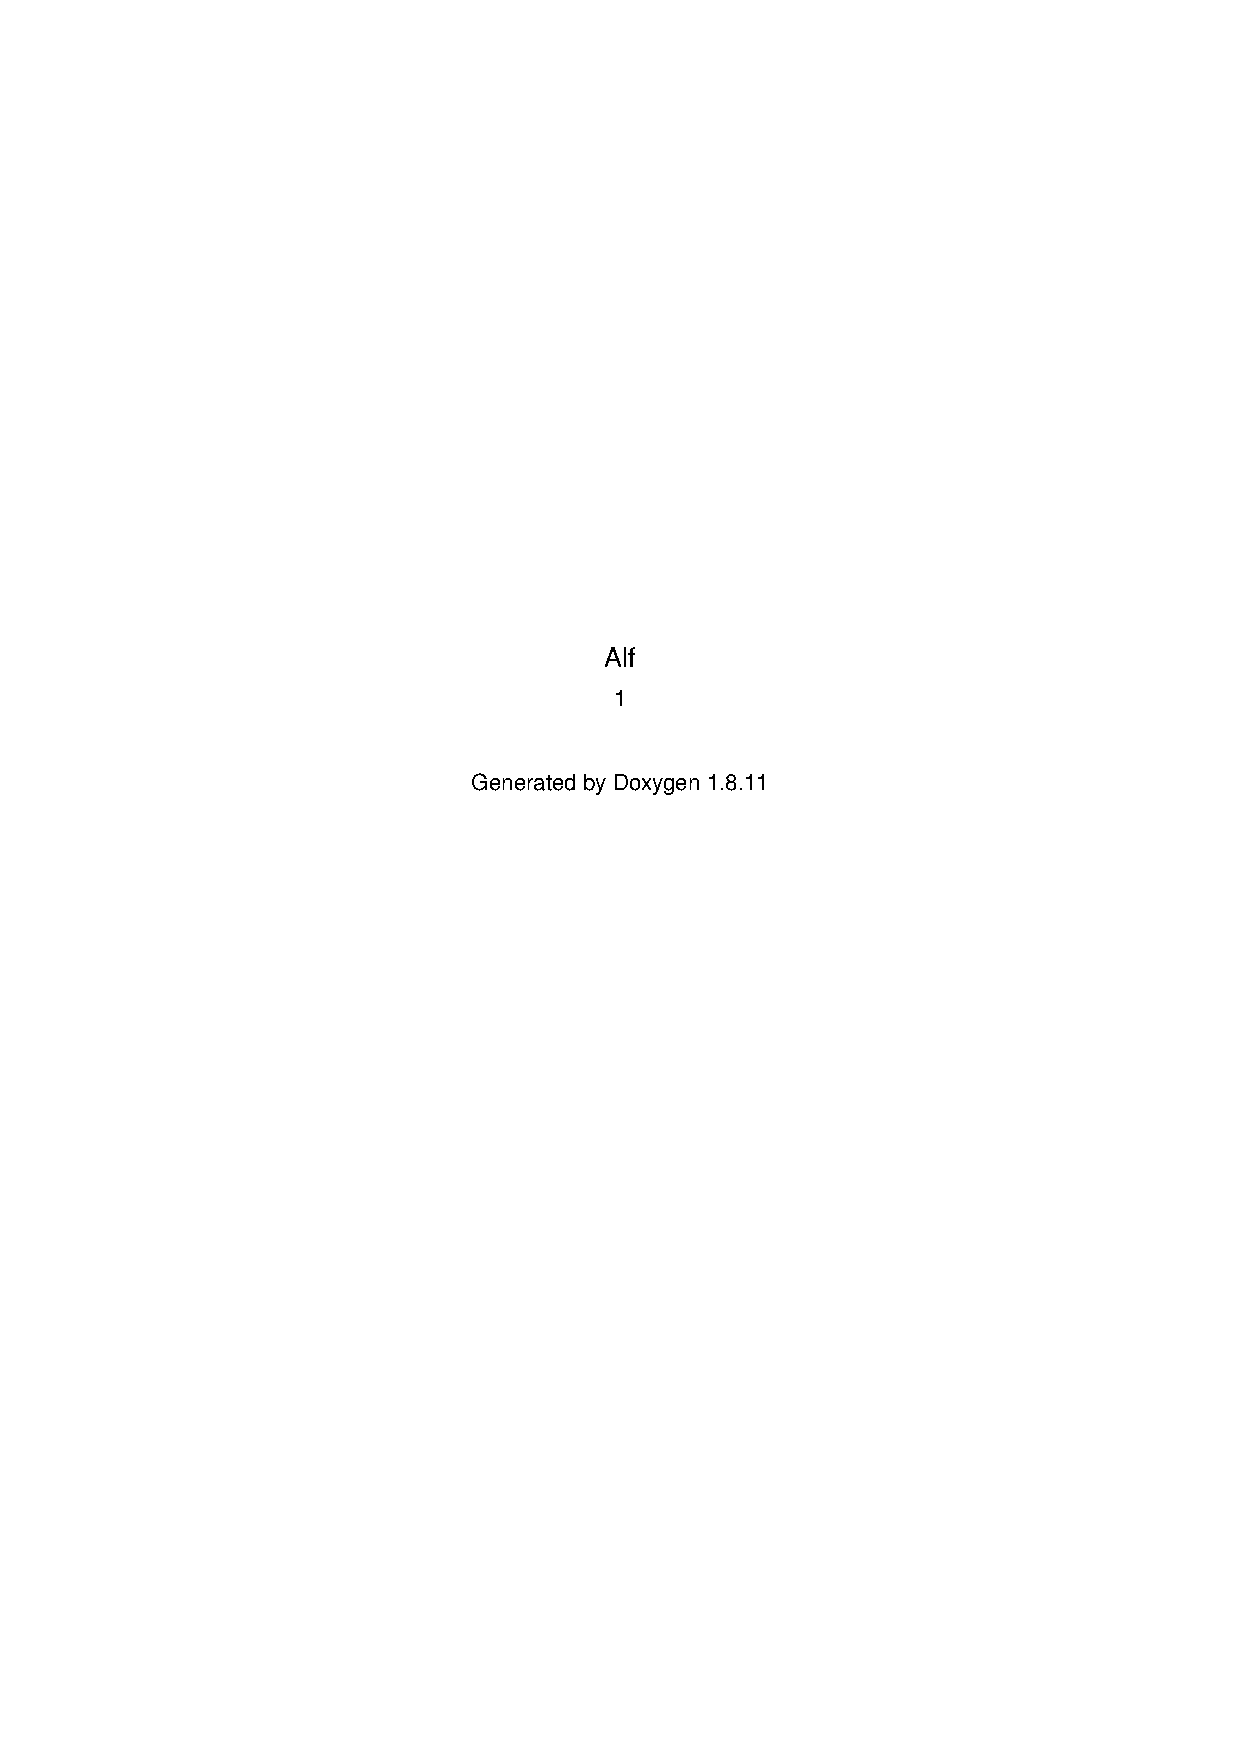
\includepdf[pages=-]{refman.pdf}

\end{document}
